\documentclass[13.6pt,a4paper]{report}

\usepackage[italian]{babel}
\usepackage[T1]{fontenc}
\usepackage[utf8]{inputenc}
\usepackage{xcolor}


\usepackage{geometry}
\geometry{
    top=2.5cm,
    bottom=2.5cm,
    left=2.8cm,
    right=2.8cm
}

\usepackage{graphicx}
\usepackage{booktabs}
\usepackage{array}
\usepackage{amsmath}
\usepackage{hyperref}
\usepackage{fancyhdr}
\usepackage{svg}
\usepackage{subcaption}
\usepackage{float}
\usepackage{placeins}

% Header simile al PDF
\pagestyle{fancy}
\fancyhf{}
\fancyhead[L]{\nouppercase{\leftmark}}
\fancyhead[R]{\thepage}
\renewcommand{\headrulewidth}{0pt}

\setlength{\fboxsep}{2pt}

\begin{document}

% Frontespizio
\begin{titlepage}
    \centering

    {\Large UNIVERSITÀ POLITECNICA DELLE MARCHE\par}
    \vspace{0.3cm}

    {\large Corso di Laurea in\par}
    {\large Ingegneria Informatica e dell'Automazione\par}

    %\vfill
    \vspace{1cm}
    
    \includesvg[width=0.6\textwidth]{images/Logo_uni.svg}

    \vspace{1.6cm}

    {\LARGE\bfseries
    SVILUPPO DI UN'INTERFACCIA GRAFICA PER UN SEMANTIC DATA LAKE
    \par}

    \vfill

    \begin{minipage}[t]{0.45\textwidth}
        \raggedright
        \Large
        \textbf{Autore:}\\
        Christian Parente\\
        Matricola 1113434
    \end{minipage}
    \hfill
    \begin{minipage}[t]{0.45\textwidth}
        \raggedleft
        \Large
        \textbf{Relatore progetto:}\\
        Prof. Emanuele Storti\\[0.5cm]

        \textbf{Docente del corso:}\\
        \Large
        Prof.ssa Claudia Diamantini
    \end{minipage}

    \vspace{3cm}

    {\large A.A. 2025/2026}

\end{titlepage}

\tableofcontents

\chapter{Introduzione}

Il progetto descritto in questa relazione prende come punto di partenza un Semantic Data Lake già esistente, le cui funzionalità sono rese disponibili attraverso un backend accessibile mediante API HTTP. Il sistema consente di gestire e analizzare differenti sorgenti dati, sfruttando informazioni semantiche per descriverne il contenuto e mettere in relazione dati provenienti da sorgenti diverse.

\noindent
L'attività svolta si è concentrata principalmente sulla realizzazione di un'interfaccia web attraverso la quale rendere tali funzionalità accessibili mediante un ambiente grafico. Durante lo sviluppo sono inoltre emerse alcune esigenze relative alla gestione delle sorgenti che hanno richiesto l'estensione e l'adattamento di alcune funzionalità del backend preesistente.

\noindent
La relazione presenta inizialmente i principali concetti teorici necessari alla comprensione del sistema e analizza successivamente l'architettura e le funzionalità del backend di partenza. Vengono quindi descritte la progettazione della soluzione, le modifiche apportate al backend e l'implementazione dell'interfaccia web. Infine, vengono discussi i risultati ottenuti e i possibili sviluppi futuri.

\noindent
Il codice sorgente del progetto e il materiale associato sono disponibili nella
\href{https://github.com/Parents99/Datalake-ui_NGD.git}{repository GitHub del progetto}.

\chapter{Cenni teorici}

\section{Semantic Data Lake}
%breve introduzione sui data lake poi spiegazione per i semantic data lake

Un Data Lake è un repository centralizzato che permette di archiviare grandi quantità di dati eterogenei, senza doverli necessariamente strutturare o trasformare preventivamente come avviene invece in un data warehouse tradizionale.
Un Data Lake, infatti, adotta frequentemente un approccio \textit{schema-on-read}: la struttura necessaria all’analisi viene applicata nel momento in cui i dati vengono utilizzati.
\noindent
Un \textbf{Semantic Data Lake} rappresenta un'evoluzione dei Data Lake in cui ai dati viene aggiunto un livello di semantica, ovvero un insieme di informazioni relative al loro significato, alle relazioni e al loro contesto.
\noindent
Questo livello permette di descrivere le sorgenti non soltanto dal punto di vista tecnico e strutturale, ma anche dal punto di vista concettuale, facilitando l'interpretazione e l'individuazione delle informazioni contenute nel Data Lake.

\noindent
La descrizione semantica può essere realizzata attraverso \textbf{metadati}, \textbf{ontologie} e \textbf{Knowledge Graph}. I metadati forniscono informazioni sulle caratteristiche delle sorgenti e dei dati contenuti. Tali informazioni possono essere organizzate all'interno di un \textbf{Metadata Graph}, una rappresentazione a grafo che descrive le sorgenti presenti nel Data Lake, i relativi attributi e le relazioni esistenti tra essi. Le ontologie, invece, definiscono i concetti appartenenti a un determinato dominio\footnote{Area tematica che raggruppa dati semanticamente correlati, definita da un vocabolario/ontologia condiviso.} e le possibili relazioni tra essi. Il Knowledge Graph consente quindi di rappresentare concretamente tali concetti e le loro relazioni sotto forma di grafo, in cui le entità sono collegate tra loro attraverso relazioni che ne descrivono il significato e il contesto. In questo modo è possibile creare collegamenti tra informazioni provenienti da sorgenti differenti e fornire una rappresentazione unificata della conoscenza associata ai dati. Dati caratterizzati da strutture o terminologie differenti possono quindi essere messi in relazione attraverso i concetti semantici a cui fanno riferimento.

\noindent
L'introduzione di questo livello consente di migliorare la ricerca, la comprensione e l'integrazione dei dati, permettendo di individuare le sorgenti sulla base del loro significato e non esclusivamente attraverso caratteristiche quali il nome o la struttura. Inoltre, una corretta descrizione dei dati contribuisce a evitare che, con l'aumento del numero e dell'eterogeneità delle sorgenti, il Data Lake diventi un insieme di dati difficilmente interpretabili e utilizzabili, fenomeno comunemente indicato come Data Swamp.

%\section{Metadata Graph}

%\section{Knowledge Graph}

\section{RDF}
%spiegare rdf poi dire anche Di sparql
\textbf{RDF (Resource Description Framework)} è un modello per rappresentare informazioni mediante triple soggetto-predicato-oggetto. Un insieme di triple forma un grafo nel quale i soggetti rappresentano risorse, i predicati esprimono proprietà o relazioni, mentre gli oggetti possono essere altre risorse oppure valori letterali. Le risorse e le proprietà sono tipicamente identificate mediante \textbf{IRI} (Internationalized Resource Identifier), che permettono di identificarle in maniera univoca e di creare collegamenti tra informazioni provenienti da sorgenti differenti.

\noindent
Per poter interrogare e recuperare le informazioni contenute in tali grafi viene utilizzato \textbf{SPARQL (SPARQL Protocol and RDF Query Language)}, un linguaggio di interrogazione specificamente progettato per dati RDF. SPARQL consente di ricercare determinati pattern di triple e di combinare più condizioni, sfruttando le relazioni presenti nel grafo per individuare le informazioni di interesse.


\chapter{Analisi del sistema preesistente}

\section{Architettura}

\noindent
Il backend del sistema è sviluppato in Python e mette a disposizione le funzionalità del Semantic Data Lake attraverso un'API HTTP realizzata mediante il framework Flask. L'architettura è organizzata in diversi layer, ciascuno responsabile di uno specifico insieme di funzionalità, in modo da separare la gestione delle richieste HTTP dalla logica applicativa e dalle operazioni sui dati.

\begin{figure}[H]
    \centering
    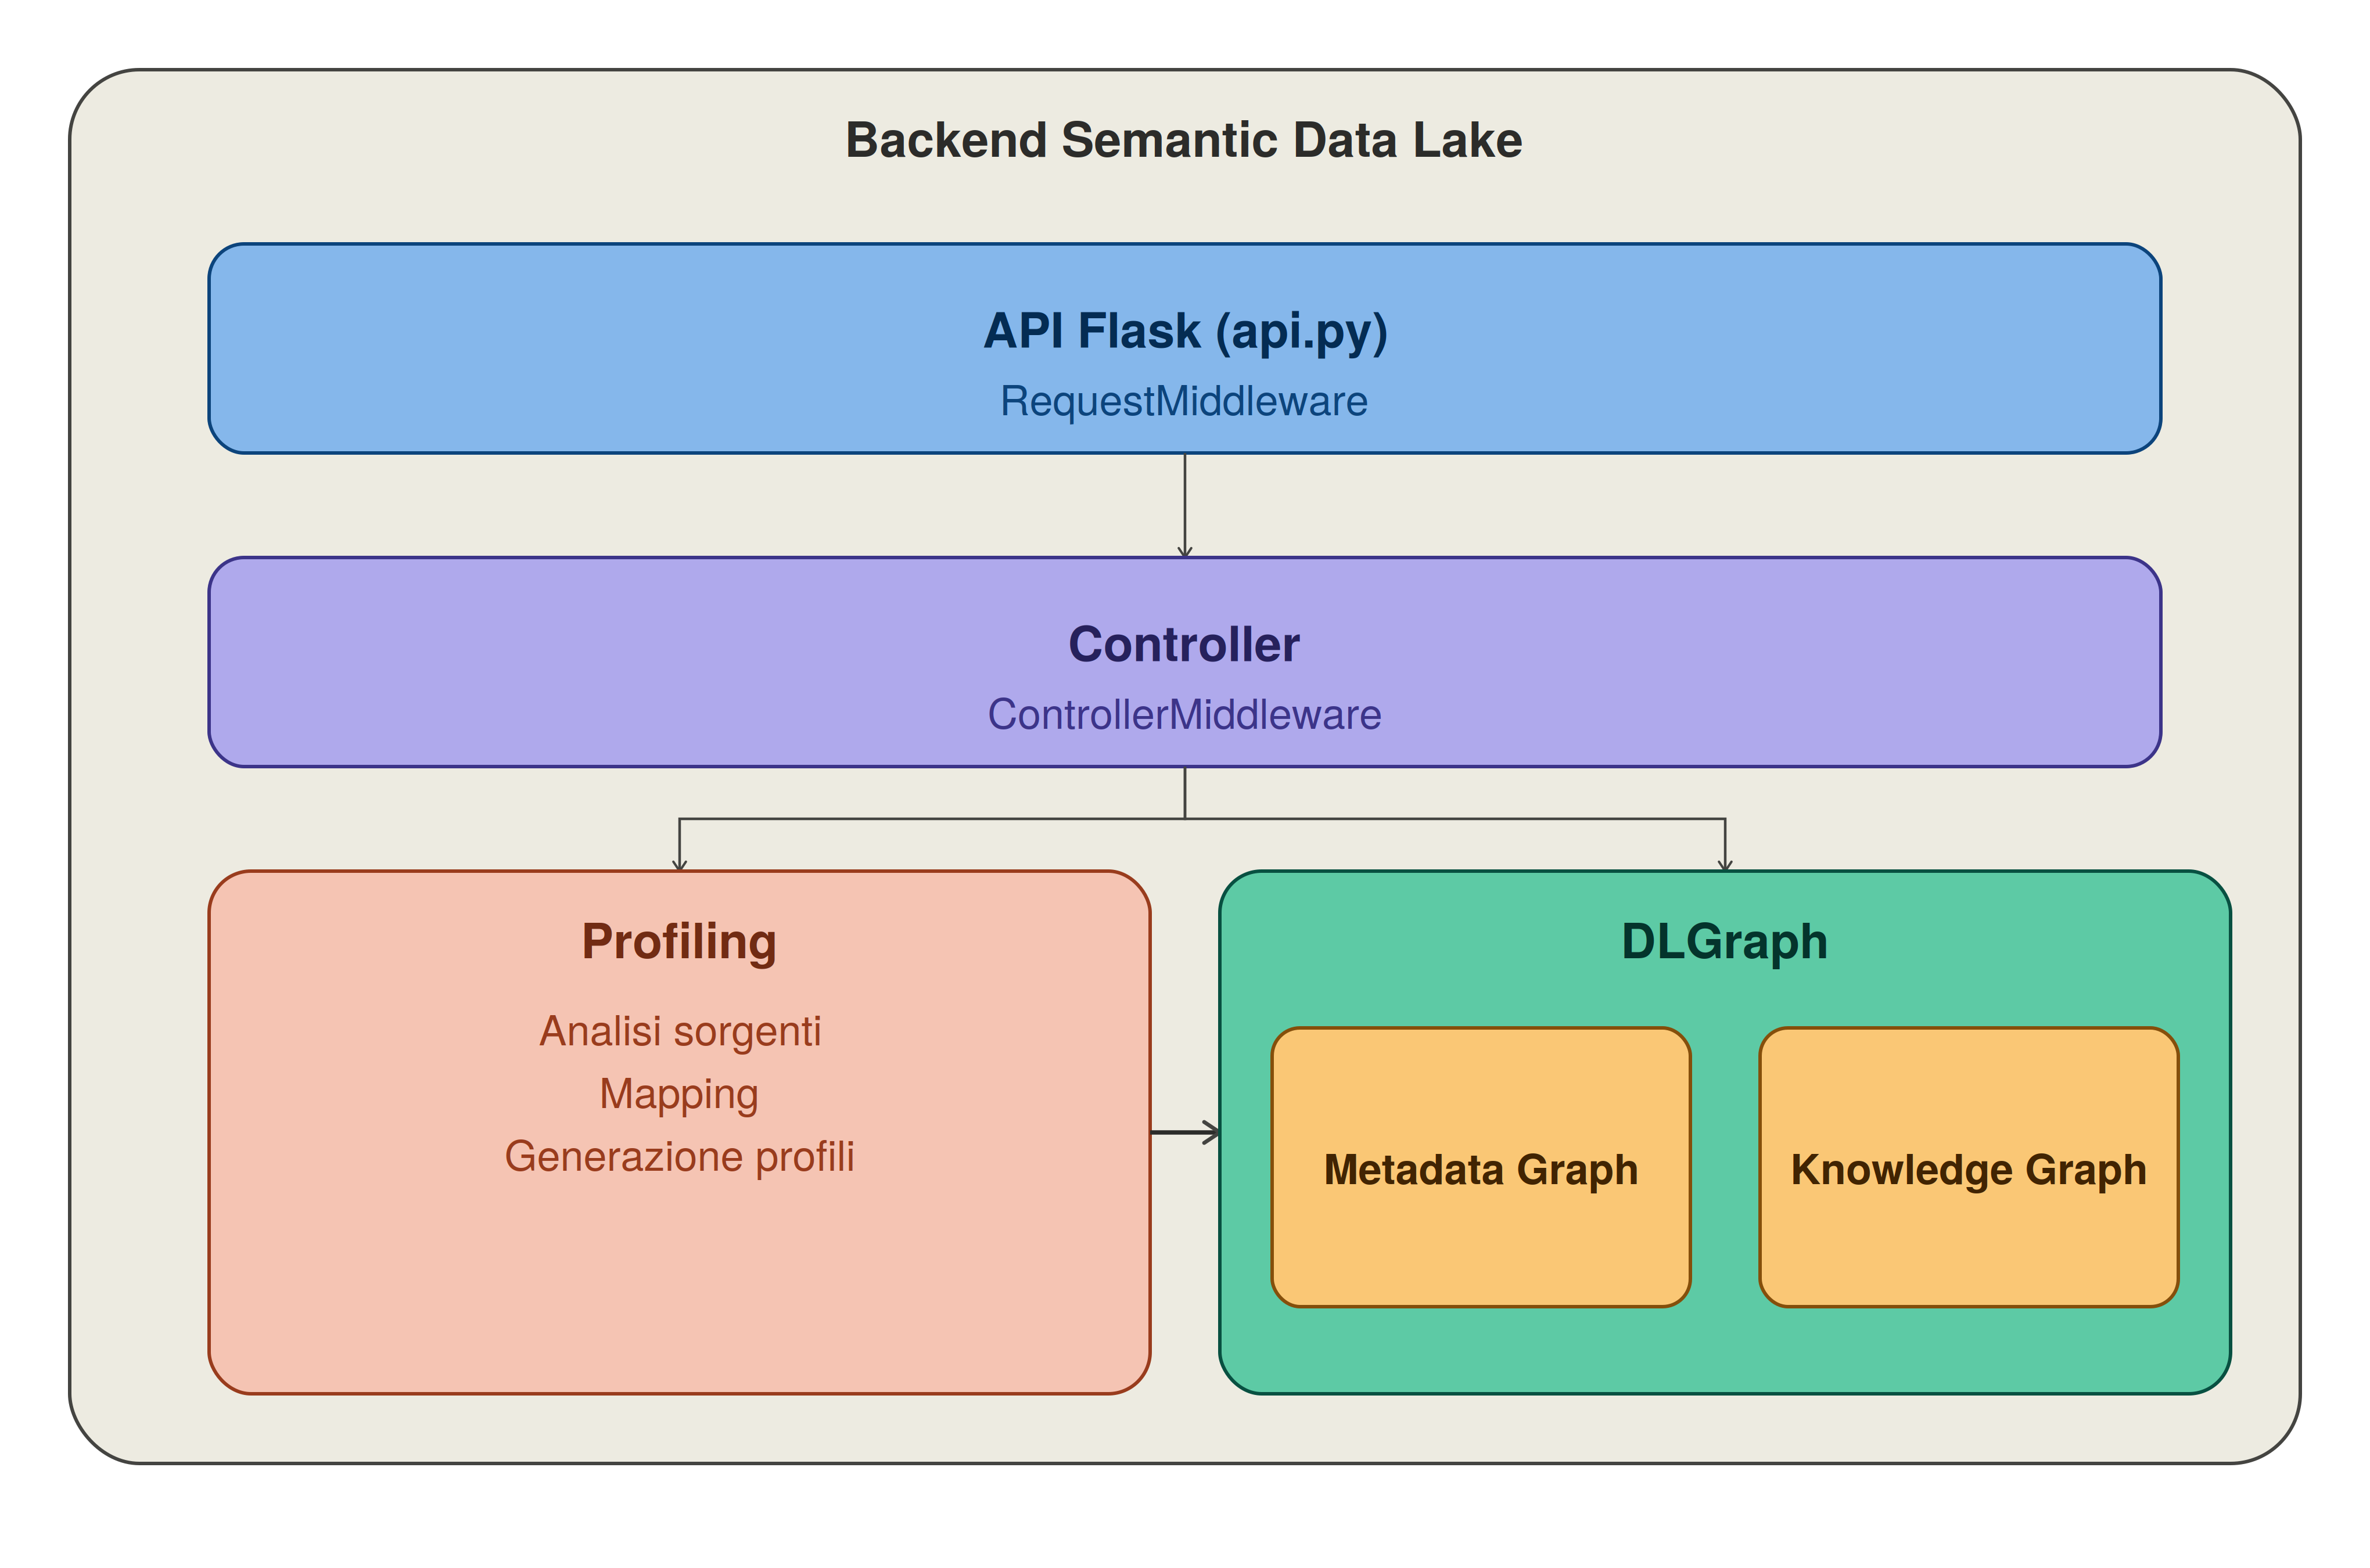
\includegraphics[width=0.75\linewidth]{images/cap. 3/architettura_data_lake_final.png}
    \caption{Architettura del sistema preesistente}
    \label{fig:placeholder}
\end{figure}

\noindent
Il punto di accesso principale alle funzionalità del sistema è rappresentato dal modulo api.py, nel quale vengono definite le diverse rotte HTTP. Questo livello riceve le richieste provenienti dal client, estrae e valida i parametri forniti e inoltra le operazioni al livello applicativo.

\noindent
La validazione delle richieste viene supportata dal middleware, che verifica la correttezza dei parametri ricevuti e gestisce alcune condizioni necessarie all'esecuzione delle operazioni, come lo stato di autenticazione dell'utente e i privilegi richiesti.

\noindent
La logica applicativa è centralizzata principalmente nella classe \textit{Controller}, che svolge il ruolo di intermediario tra l'API e i componenti responsabili della gestione del Data Lake. Il controller verifica le condizioni necessarie all'esecuzione delle operazioni e coordina le funzionalità relative agli utenti, alle sorgenti e ai grafi utilizzati dal sistema.

\noindent
La rappresentazione semantica dei dati è gestita attraverso due componenti principali: il \textbf{Metadata Graph} e il \textbf{Knowledge Graph}. Il primo mantiene le informazioni relative alle sorgenti caricate nel Data Lake e ai relativi profili, mentre il secondo rappresenta la conoscenza utilizzata dal sistema per organizzare e mettere in relazione semanticamente i dati. La classe \textit{DLGraph} fornisce le operazioni che richiedono l'interazione tra questi due livelli.

\noindent
Sono inoltre presenti moduli dedicati alle operazioni di profiling, responsabili dell'elaborazione delle sorgenti, della generazione dei relativi profili e delle operazioni di caricamento e mount.

% client -> api flask -> Middleware -> Controller -> moduli per la gestione del data lake
%**** schema del flusso delle richieste / diagramma dell'architettura ****



\section{Funzionalità}

\subsection{Gestione degli utenti}
%parlare della gestione degli utenti e dei ruoli

Il backend mette a disposizione funzionalità per la registrazione, l'autenticazione e la disconnessione degli utenti. Le operazioni sono esposte rispettivamente attraverso le rotte \colorbox{gray!15}{/signin}, \colorbox{gray!15}{/login}, \colorbox{gray!15}{/logout}. Le informazioni relative agli utenti sono memorizzate in un file CSV, nel quale vengono conservati il nome utente, il ruolo e l'hash della password.

\noindent
In seguito al login, le informazioni relative all'utente autenticato vengono mantenute dal backend per tutta la durata della sessione applicativa e utilizzate nelle richieste successive per identificarlo e verificarne i privilegi. Il logout determina invece la cancellazione di tali informazioni e la conclusione della sessione corrente.

\noindent
Il sistema distingue tra utenti ordinari e amministratori. Gli utenti possono operare sulle proprie sorgenti, mentre le rotte appartenenti allo spazio \colorbox{gray!15}{/admin} consentono all'amministratore di eseguire operazioni anche sulle risorse appartenenti agli altri utenti.


\noindent

\subsection{Gestione delle sorgenti}


La rotta \colorbox{gray!15}{/mount} permette di integrare una sorgente nel Data Lake. Si fornisce un file CSV nella richiesta HTTP e il file viene salvato su un percorso dedicato alle sorgenti di ogni utente. A questo punto si avvia il processo di profiling, attraverso il quale vengono analizzati la struttura e il contenuto della sorgente e vengono generate le informazioni necessarie alla sua rappresentazione all'interno del sistema. I risultati ottenuti vengono utilizzati per aggiornare il Metadata Graph e, quando possibile, mettere in relazione i dati della sorgente con le informazioni presenti nel Knowledge Graph.

\noindent
Il sistema supporta inoltre l'operazione di \textbf{remount}, che consente di elaborare nuovamente una sorgente già montata modificando i parametri utilizzati per il profiling. In questo caso, le informazioni precedentemente associate alla sorgente vengono aggiornate sulla base della nuova elaborazione, senza richiedere un nuovo caricamento del file.

\noindent
Durante l'operazione di mount è possibile specificare alcuni parametri che influenzano il processo di profiling della sorgente. In particolare, stringProcessing stabilisce se eseguire le operazioni di profiling specifiche per i dati testuali, mentre frequentWords definisce il numero di parole più frequenti da considerare durante tale analisi. Il parametro maxCategories indica il numero massimo di valori distinti entro il quale un dominio viene considerato categorico, mentre dateThreshold definisce la soglia utilizzata per il riconoscimento dei valori di tipo data.

\noindent
Gli stessi parametri possono essere specificati durante il remount, consentendo di elaborare nuovamente una sorgente già presente nel Data Lake utilizzando una configurazione differente.

\noindent
L'operazione inversa è fornita da  \colorbox{gray!15}{/unmount}, che permette di rimuovere una sorgente precedentemente montata dal Data Lake. L’operazione elimina il file associato alla sorgente e rimuove dal Metadata Graph i relativi metadati.

\noindent
Infine, si ha la rotta \colorbox{gray!15}{/sources} che permette di ottenere la lista delle sorgenti montate all'interno del Data lake.

\noindent
%\subsection*{Reset metadati}
Il backend mette inoltre a disposizione la rotta \colorbox{gray!15}{/clean}, che consente di effettuare una pulizia completa del livello dei metadati relativo all'utente autenticato. L'operazione rimuove dal Metadata Graph tutte le sorgenti appartenenti all'utente e i metadati ad esse associati. Prima di procedere è richiesta una conferma esplicita tramite un apposito parametro della richiesta, in modo da evitare l'esecuzione accidentale dell'operazione.


\subsection{Analisi delle sorgenti}
Una volta effettuato il mount, il backend mette a disposizione diverse funzionalità per analizzare le sorgenti e le informazioni generate durante il processo di profiling.

\subsubsection*{Describe}
La rotta \colorbox{gray!15}{/describe} fornisce una descrizione generale della sorgente, riportando informazioni quali l'utente che ne ha effettuato il caricamento, la data di caricamento, il numero di elementi e il numero di domini individuati. Per ciascun dominio viene inoltre indicato se è stato associato a un livello del Knowledge Graph e, in caso affermativo, viene calcolato il relativo grado di completezza.

\noindent
Queste informazioni forniscono quindi una vista generale della sorgente e permettono di individuare i domini per i quali è stata stabilita una corrispondenza con la struttura semantica rappresentata nel Knowledge Graph.

\subsubsection*{Profile}
La rotta \colorbox{gray!15}{/profile} permette invece di accedere alle informazioni di profiling associate ai domini di una sorgente. È possibile ottenere il profilo di tutti i domini oppure selezionarne uno specifico. Per i domini associati a un livello del Knowledge Graph è inoltre disponibile un'operazione di roll-up, che consente di ottenere il profilo rispetto ai livelli superiori della gerarchia semantica. Il roll-up non è invece applicabile ai domini per i quali non è stata individuata una corrispondenza nel Knowledge Graph.

\noindent
Le informazioni restituite dipendono dalle caratteristiche del dominio analizzato e possono quindi assumere forme differenti in funzione della tipologia dei dati, ad esempio numerici, categorici, testuali o temporali. Il profilo rappresenta in questo modo una descrizione delle principali caratteristiche individuate durante la fase di profiling della sorgente.


\subsubsection*{Estimate}
La rotta \colorbox{gray!15}{/estimate} permette di confrontare due sorgenti sulla base dei livelli del Knowledge Graph a cui sono stati associati i rispettivi domini. Il confronto viene effettuato sui livelli comuni alle due sorgenti, rappresentando la distribuzione dei valori dei relativi domini mediante vettori e calcolandone la similarità del coseno. Per ciascun livello comune viene quindi restituito un valore percentuale di similarità, insieme ai domini delle due sorgenti coinvolti nel confronto.

\noindent
Il confronto viene quindi effettuato sulla base della corrispondenza semantica dei domini, utilizzando i livelli condivisi del Knowledge Graph come riferimento comune tra le due sorgenti.


\subsection{Funzionalità amministrative}
%da vedere se metterlo, c'è anche la parte di eliminazione degli utenti, magari spiegare che c'è il corrispettivo di ogni rotta per l'admin che permette di effettuare le operazioni per conto di un altro utente

%\subsubsection*{Query}
%ovviamente specificare che è per admin

%\subsection*{Eliminazione utenti}

\noindent
Oltre agli endpoint disponibili agli utenti ordinari, il backend espone le corrispondenti versioni amministrative. Queste mantengono un funzionamento analogo, ma consentono di specificare l'utente sul quale eseguire la richiesta, permettendo quindi all'amministratore di intervenire anche sulle risorse appartenenti ad altri utenti.

\noindent
Sono inoltre disponibili ulteriori rotte specifiche per l'utente amministratore:
\begin{itemize}
    \item la rotta \colorbox{gray!15}{/admin/query}, che permette di eseguire interrogazioni SPARQL dirette sui grafi RDF gestiti dal sistema, specificando la query e il grafo di destinazione (Metadata Graph o Knowledge Graph). A differenza delle altre funzionalità, che espongono operazioni predefinite sui dati, questa rotta offre un meccanismo di interrogazione più flessibile, dando all'amministratore accesso diretto alle informazioni contenute nei grafi.
    
    \item la rotta \colorbox{gray!15}{/admin/deleteUser}, che permette di eliminare un utente registrato nel sistema. L'operazione non si limita alla rimozione delle credenziali dal file utilizzato per la gestione degli utenti, ma provvede anche alla pulizia delle risorse associate, eliminando le sorgenti e i relativi metadati dal sistema.

    \item la rotta \colorbox{gray!15}{/admin/users}, che permette di ottenere l'elenco degli utenti registrati nel sistema. Tale funzionalità viene utilizzata dall'interfaccia amministrativa per consentire la selezione dell'utente sul quale eseguire le diverse operazioni e per visualizzare gli account disponibili nella sezione dedicata alla gestione degli utenti.
\end{itemize}


%\section{Limiti}
% da vedere se metterla o no
% se si mette aggiungere la parte della risoluzione degli errori (da valutare)


\chapter{Progettazione della soluzione}

\section{Analisi dei requisiti}
%parlare della gestione dei ruoli
% parlare delle funzionalità che devono essere implementate (che sarebbero quelle del backend) 

L'obiettivo principale del progetto consiste nella realizzazione di un'interfaccia web che permetta di accedere in maniera semplice e intuitiva alle funzionalità messe a disposizione dal backend del Semantic Data Lake.

\noindent
L'applicazione deve consentire agli utenti di autenticarsi e utilizzare, attraverso l'interfaccia grafica, le principali operazioni offerte dalle API per la gestione delle sorgenti nel Data lake.

\noindent
Un ulteriore requisito riguarda la distinzione tra utenti ordinari e amministratori. L'interfaccia deve tenere conto del ruolo dell'utente autenticato e rendere disponibili le relative funzionalità. Gli utenti ordinari possono esclusivamente operare sulle proprie sorgenti, mentre gli amministratori possono sfruttare le operazioni aggiuntive messe a disposizione dalle rotte dedicate del backend, intervenendo anche sulle sorgenti appartenenti agli altri utenti e accedendo alle funzionalità di amministrazione del sistema.

\noindent
Durante lo sviluppo è inoltre emersa l'esigenza di rendere più flessibile la gestione delle sorgenti. Nel sistema originario, il caricamento e l'integrazione di una sorgente nel Data lake erano direttamente associati ad un'unica operazione di mount. È stata quindi introdotta la possibilità di caricare e memorizzare una sorgente senza integrarla immediatamente nel Data Lake, permettendo all'utente di effettuare il mount in un momento successivo. Tale requisito ha comportato l'estensione del backend e la modifica di alcune delle funzionalità preesistenti, descritte nel capitolo successivo.

\section{Architettura}
%aggiungere le tecnologie utilizzate
%alla fine del capitolo (o in una section differente aggiungere 
%\section{Gestione delle sorgenti}

La soluzione è stata progettata secondo un'architettura client-server, mantenendo una netta separazione tra il backend del Semantic Data Lake e l'interfaccia web sviluppata. Il frontend rappresenta il livello di presentazione del sistema e costituisce il principale punto di interazione con l'utente, mentre il backend mantiene la responsabilità della logica applicativa, della gestione della sessione, delle sorgenti e dell'accesso ai grafi utilizzati dal Data Lake. La comunicazione tra i due livelli avviene attraverso le API HTTP esposte dal backend. Le azioni effettuate dall'utente tramite l'interfaccia vengono tradotte in richieste verso i relativi endpoint; le risposte ricevute vengono successivamente elaborate dal frontend e utilizzate per aggiornare le informazioni visualizzate. L'interfaccia e il backend vengono eseguiti come applicazioni separate, permettendo di mantenere indipendenti i rispettivi livelli.

%*** diagramma dell'architettura che illustra la  comunicazione tra frontend e backend ***

\noindent
Il frontend è stato sviluppato utilizzando React e TypeScript, con Vite come strumento di sviluppo e build e Tailwind CSS per la definizione dell'interfaccia grafica. La navigazione tra le diverse funzionalità è gestita tramite React Router, organizzando l'applicazione in viste distinte e separando le funzionalità disponibili agli utenti ordinari da quelle riservate agli amministratori. 

\noindent
L'accesso al backend è centralizzato in un livello dedicato alla comunicazione con le API, realizzato mediante Axios. Tale livello raccoglie le operazioni necessarie per l'autenticazione, la gestione delle sorgenti e l'esecuzione delle diverse funzionalità offerte dal backend, separando la logica relativa alle richieste HTTP dai componenti dell'interfaccia.

\noindent
La gestione dello stato globale dell'utente autenticato è affidata a Zustand, mentre le informazioni relative all'autenticazione vengono conservate nel browser per ripristinare lo stato dell'interfaccia dopo il ricaricamento della pagina.


\chapter{Estensione del backend}

Il backend descritto nei capitoli precedenti ha costituito il punto di partenza per lo sviluppo del progetto. Durante la realizzazione dell'interfaccia e le successive fasi di revisione è emersa la necessità di estenderne alcune funzionalità, sia per supportare nuove modalità di gestione delle sorgenti sia per adattare le operazioni esistenti alle esigenze dell'applicazione sviluppata.

\noindent
Gli interventi effettuati hanno riguardato principalmente l'introduzione di nuove funzionalità per la gestione delle sorgenti non ancora montate e la modifica di alcuni endpoint già presenti. 


\section{Funzionalità aggiuntive}
%parlare dei nuovi endpoint
% fare schema sulla gestione delle sorgenti (ciclo di vita)

Per soddisfare il requisito descritto nel capitolo precedente, è stato introdotto un meccanismo di upload indipendente dal mount, attraverso il quale una sorgente può essere caricata e memorizzata sul server senza avviarne immediatamente l'elaborazione. In questo modo l'utente può caricare preventivamente una o più sorgenti e decidere successivamente quali sottoporre al processo di mount.

\noindent
Le sorgenti caricate con questa modalità vengono memorizzate nella directory datasets/to\_mount, utilizzata per raccogliere i file in attesa di essere montati. Al suo interno viene mantenuta una directory separata per ciascun utente, in modo da distinguere le rispettive sorgenti. Il ciclo di vita di un file può quindi prevedere uno stato intermedio tra il caricamento e l'integrazione nel Data Lake.

%*** schema sulla gestione delle sorgenti (ciclo di vita) ***
%\includegraphics[width=0.55\textwidth]{}

\begin{figure}
    \centering
    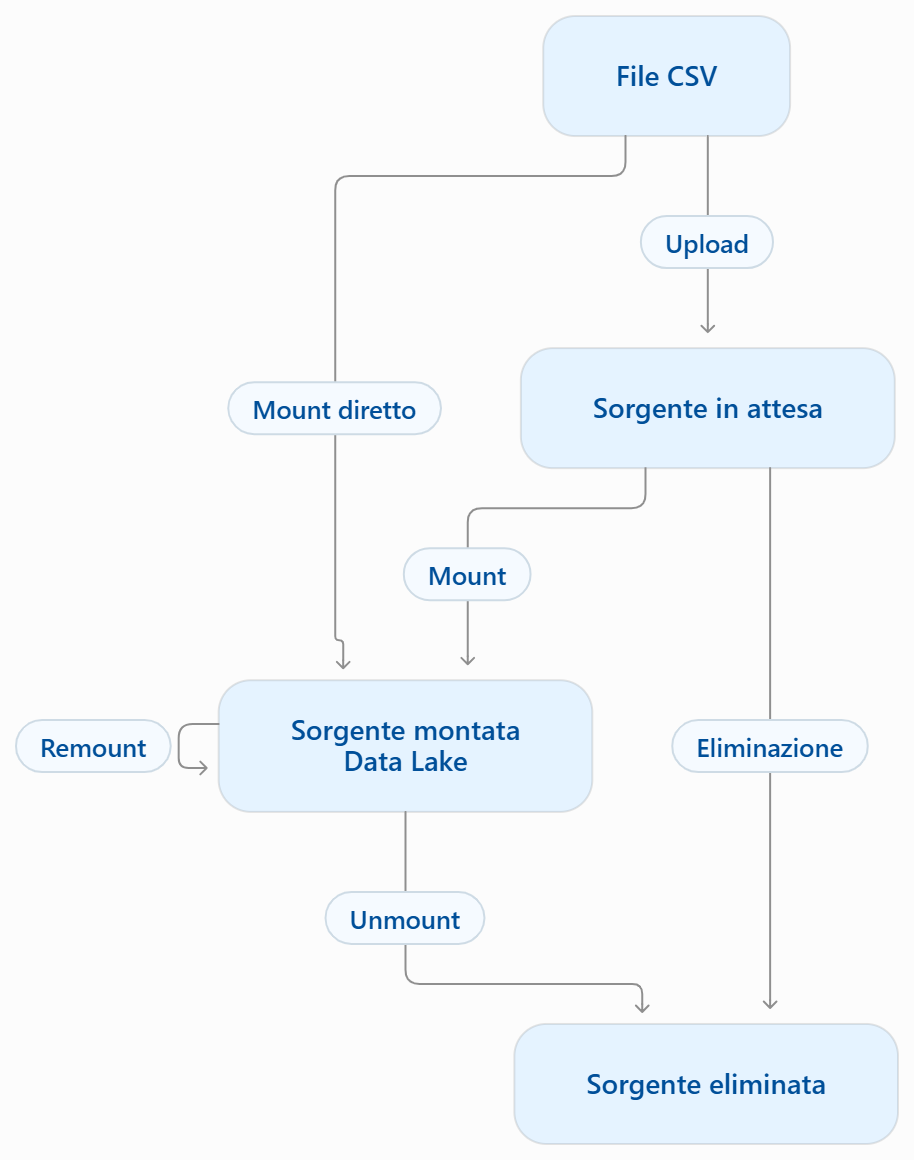
\includegraphics[width=0.55\linewidth]{images/cap. 5/ciclo_di_vita_sorgenti_2.png}
    \caption{Flusso di gestione delle sorgenti}
    \label{fig:placeholder}
\end{figure}

\subsection*{Upload delle sorgenti}

La nuova rotta \colorbox{gray!15}{/ POST upload} consente all'utente autenticato di inviare una sorgente al server senza avviarne il mount. Prima del salvataggio vengono effettuati i controlli necessari sul file e viene verificata l'eventuale presenza di una sorgente con lo stesso nome tra quelle già caricate dall'utente. In assenza di conflitti, il file viene memorizzato nella relativa directory all'interno di datasets/to\_mount/<nome\_utente>.

\noindent
Per mantenere le stesse possibilità di gestione anche per gli amministratori è stata introdotta la rotta \colorbox{gray!15}{POST /admin/upload}. Il funzionamento è analogo, con la differenza che l'amministratore può specificare l'utente al quale associare la sorgente, determinando quindi la directory nella quale questa viene memorizzata.

\noindent
Inoltre, per consentire l'accesso alle sorgenti precedentemente caricate sono state introdotte le rotte \colorbox{gray!15}{GET /uploads} e \colorbox{gray!15}{ GET /admin/uploads}. La prima restituisce l'insieme dei file in attesa di mount appartenenti all'utente autenticato, mentre la seconda permette all'amministratore di ottenere quelli relativi a uno specifico utente.

\noindent
Queste operazioni permettono al frontend di rappresentare separatamente le sorgenti già integrate nel Data Lake e quelle semplicemente memorizzate sul server, rendendo possibile la successiva selezione dei file sui quali eseguire il mount.


\subsection*{Eliminazione delle sorgenti non montate}

È stata infine introdotta la possibilità di eliminare una sorgente precedentemente caricata ma non ancora montata. La rotta \colorbox{gray!15}{DELETE /uploads/<filename> } rimuove il file dalla directory dell'utente, dopo averne verificato l'esistenza. Anche in questo caso è disponibile una corrispondente operazione amministrativa, \colorbox{gray!15}{DELETE /admin/uploads/<filename> }, che consente di eseguire la stessa operazione sulle sorgenti appartenenti a uno specifico utente.

\section{Modifiche degli endpoint esistenti}

%\section{Integrazione delle funzionalità nell'interfaccia}
%da vedere se mettere questa sezione, perché se ne parla poi nell'implementazione (magari si può fare un riferimento quando si parla dell'upload ecc.

L'introduzione della possibilità di caricare una sorgente senza effettuarne immediatamente il mount ha richiesto di adattare l'operazione di mount già presente nel backend. Il comportamento originario è stato mantenuto, consentendo quindi di continuare a inviare un nuovo file ed eseguirne direttamente l'elaborazione, affiancandogli la possibilità di operare sulle sorgenti precedentemente caricate sul server.

\noindent
L'endpoint /mount è stato quindi esteso per distinguere tre differenti modalità operative: il mount diretto di una nuova sorgente, il remount di una sorgente già integrata nel Data Lake e il mount di una sorgente precedentemente caricata tramite la funzionalità di upload. La modalità richiesta viene determinata attraverso i parametri forniti nella richiesta, mantenendo in un unico endpoint le diverse operazioni relative al processo di mount.

\noindent
Nel caso di una sorgente precedentemente caricata, il backend individua il file nella directory to\_mount relativa all'utente e ne crea una copia nella directory destinata alle sorgenti montate. Il file viene quindi sottoposto al normale processo di elaborazione e integrazione nel Data Lake. Solamente in seguito al completamento corretto dell'operazione la sorgente originale viene rimossa da to\_mount, completandone il passaggio dallo stato di sorgente caricata a quello di sorgente montata.

\noindent
Questo viene fatto per preservare la sorgente originale in caso di errore durante il mount; qualora l'elaborazione non venga completata correttamente, la copia eventualmente creata nella directory delle sorgenti montate viene rimossa, mentre il file presente in to\_mount rimane disponibile per un successivo tentativo.


\chapter{Implementazione}

Il frontend è stato sviluppato adottando una struttura modulare, con l'obiettivo di separare le diverse responsabilità dell'applicazione e favorire il riutilizzo dei componenti. Il codice è organizzato in pagine, corrispondenti alle principali viste dell'interfaccia, e componenti riutilizzabili condivisi tra le diverse funzionalità.

\noindent
La logica relativa alla comunicazione con il backend è mantenuta separata dai componenti grafici attraverso un livello dedicato alle chiamate API. Analogamente, la navigazione e la gestione dello stato condiviso dell'applicazione sono affidate a moduli specifici, evitando di concentrare all'interno dei singoli componenti responsabilità non direttamente legate alla presentazione e all'interazione con l'utente.

\section{Autenticazione e sessione}
L'accesso alle funzionalità dell'applicazione è subordinato all'autenticazione dell'utente. Il frontend mette a disposizione le interfacce per effettuare il login e la registrazione, attraverso le quali vengono raccolte le credenziali e inviate le relative richieste al backend. In caso di autenticazione completata correttamente, l'utente viene indirizzato verso l'interfaccia principale dell'applicazione.

\noindent
Le informazioni necessarie a rappresentare lo stato di autenticazione sono gestite centralmente mediante uno store Zustand. Lo store mantiene lo username dell'utente autenticato, il relativo ruolo e lo stato di autenticazione, rendendo tali informazioni disponibili ai diversi componenti dell'applicazione senza la necessità di propagarle manualmente tra le diverse pagine.

\noindent
Lo stato viene inoltre mantenuto nel localStorage del browser, consentendo al frontend di ripristinare le informazioni relative all'utente in seguito al ricaricamento della pagina. L'operazione di logout provvede invece a rimuovere lo stato memorizzato e a riportare l'applicazione alla schermata di autenticazione.

\noindent
L'accesso alle pagine dell'applicazione è controllato attraverso il sistema di routing. Le rotte che richiedono un utente autenticato sono protette mediante un apposito componente, che verifica lo stato dell'utente prima di consentire la visualizzazione della pagina richiesta. L'interfaccia distingue inoltre tra utente ordinario e amministratore, rendendo disponibili a quest'ultimo le viste e le funzionalità amministrative previste dall'applicazione. Il controllo effettivo delle autorizzazioni rimane comunque responsabilità del backend.

\noindent
La registrazione di un nuovo utente viene gestita attraverso un'apposita schermata, nella quale vengono richiesti username e password. I dati inseriti vengono inviati all'endpoint /signin del backend, che si occupa della validazione delle credenziali e della creazione del nuovo utente.


\begin{figure}[h]
    \centering

    \begin{subfigure}[b]{0.5\textwidth}
        \centering
        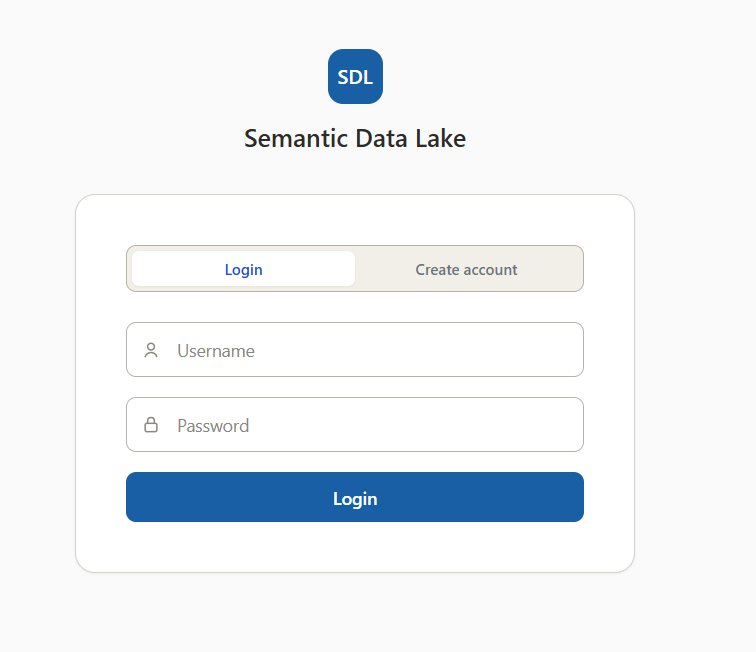
\includegraphics[width=\textwidth]{images/cap. 6/login.PNG}
        \caption{Pagina di login}
        \label{fig:immagine1}
    \end{subfigure}
    \hfill
    \begin{subfigure}[b]{0.48\textwidth}
        \centering
        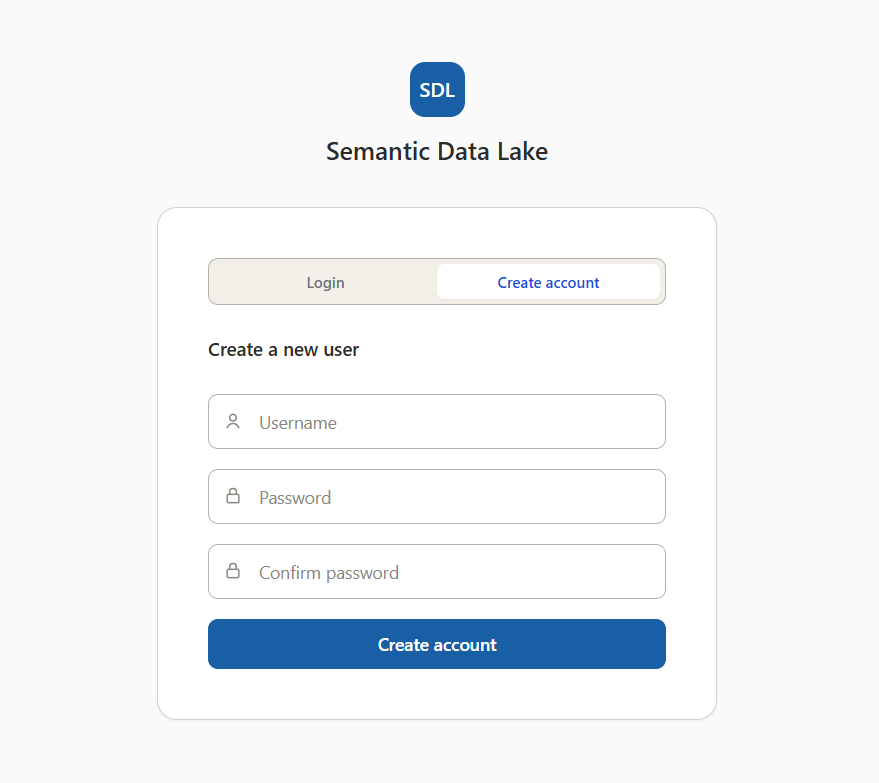
\includegraphics[width=\textwidth]{images/cap. 6/signin.PNG}
        \caption{Pagina per la registrazione di un nuovo account}
        \label{fig:immagine2}
    \end{subfigure}

\end{figure}

\section{Layout e navigazione}

Una volta effettuata l'autenticazione, l'utente accede all'interfaccia principale dell'applicazione, organizzata attraverso un layout comune alle diverse funzionalità. Tale struttura permette di mantenere invariati gli elementi principali dell'interfaccia durante la navigazione, modificando solamente il contenuto della vista selezionata.

\noindent
La navigazione tra le diverse funzionalità avviene principalmente attraverso una barra laterale, dalla quale è possibile accedere alle varie pagine. Il contenuto centrale dell'interfaccia viene aggiornato in base alla rotta selezionata, consentendo di passare tra le diverse operazioni senza modificare la struttura generale dell'applicazione.

\noindent
Le voci disponibili nella navigazione dipendono dal tipo di utente autenticato, l'interfaccia amministrativa rende disponibili anche le operazioni riservate all'amministratore come ad esempio la console per SPARQL.


\section{Gestione delle sorgenti}
%\section{Pagina Sources}
%\section{Upload}
%\section{Mount e remount}

La gestione delle sorgenti è organizzata principalmente attraverso due pagine dell'interfaccia: la pagina \textbf{Sources}, dedicata alla visualizzazione delle sorgenti e all'accesso alle operazioni disponibili, e la pagina \textbf{Mount}, utilizzata per configurare ed eseguire le diverse modalità di mount.

\noindent
La pagina Sources distingue le sorgenti associate all'utente in due sezioni separate: le sorgenti già montate e quelle precedentemente caricate sul server e ancora in attesa di mount. All'interno di ciascuna sezione, ogni sorgente è rappresentata mediante una card contenente le relative informazioni e i pulsanti corrispondenti alle operazioni disponibili. Le azioni mostrate dipendono quindi dallo stato della sorgente: per quelle già montate sono disponibili le operazioni previste per la loro consultazione e gestione, mentre per le sorgenti in attesa è possibile avviare il mount oppure eliminare il file caricato.

\noindent
Nella parte superiore della pagina Sources è inoltre presente il pulsante dedicato all'upload di nuove sorgenti. La selezione del pulsante apre una finestra di dialogo attraverso la quale è possibile selezionare o trascinare un file CSV. Il caricamento memorizza la sorgente sul server senza avviarne immediatamente il processo di integrazione; al termine dell'operazione il nuovo file viene quindi visualizzato nella sezione dedicata alle sorgenti in attesa di mount.


%**** screen schermata sources  ****
\begin{figure}[!ht]
    \centering
    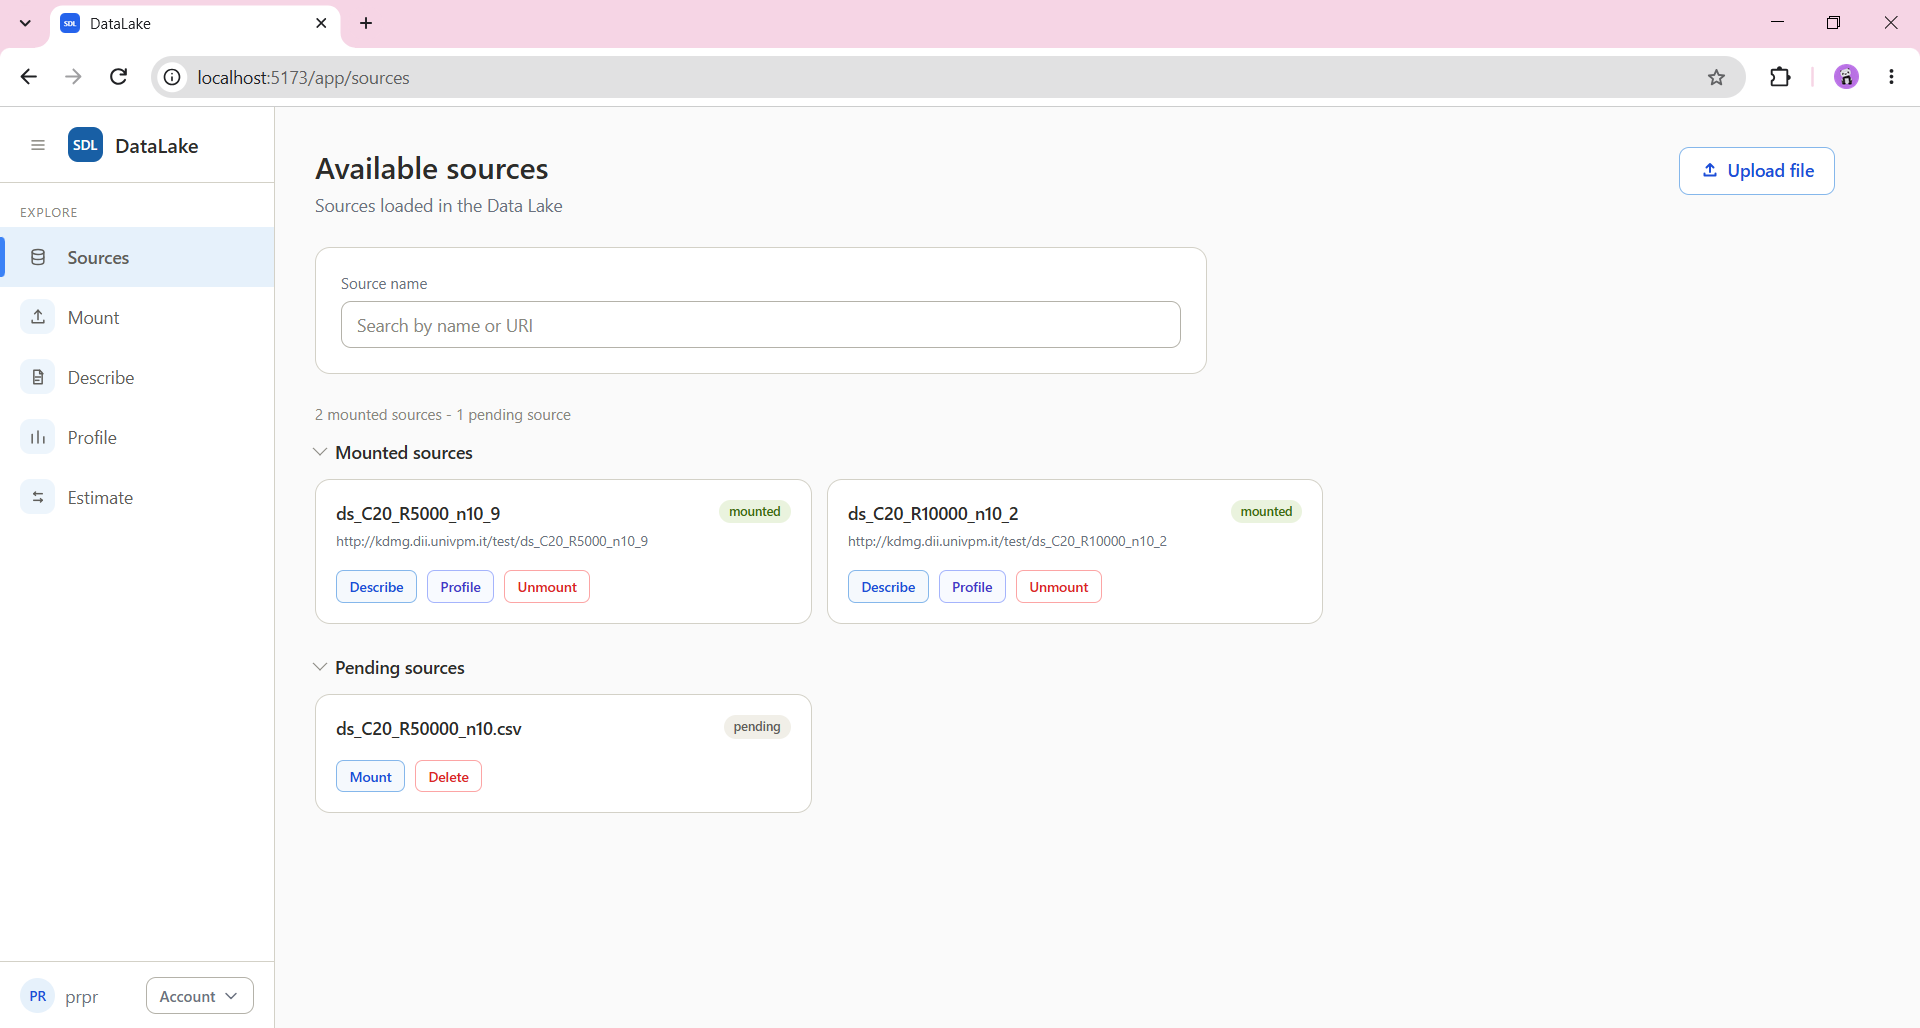
\includegraphics[width=0.9\linewidth]{images/cap. 6/sources.PNG}
    \caption{Pagina di gestione delle sorgenti}
    \label{fig:placeholder}
\end{figure}


\noindent
Le operazioni di mount sono raccolte in un'unica pagina dedicata. Un apposito selettore permette di scegliere tra tre modalità: il mount diretto di un nuovo file locale, il remount di una sorgente già integrata e il mount di una sorgente precedentemente caricata sul server. La stessa interfaccia viene quindi riutilizzata per configurare le diverse operazioni, adattando i dati richiesti in funzione della modalità selezionata.

\FloatBarrier

\noindent
Nel caso del mount diretto, l'utente seleziona il file da elaborare e configura i parametri necessari al processo. Per il remount viene invece selezionata una delle sorgenti già montate, mentre nella modalità dedicata alle sorgenti in attesa è possibile scegliere uno dei file precedentemente caricati tramite upload. In tutti i casi, la pagina consente di specificare i parametri di elaborazione previsti dal backend prima di avviare l'operazione.


\noindent
L'accesso alla modalità appropriata può avvenire anche direttamente dalla pagina Sources attraverso i pulsanti presenti nelle card. In questo modo l'utente può selezionare una sorgente e raggiungere la pagina Mount già nel contesto dell'operazione richiesta, mantenendo comunque la possibilità di passare tra le diverse modalità attraverso il selettore presente nella pagina.

%*** screen schermata mount ***

\begin{figure}[h]
    \centering

    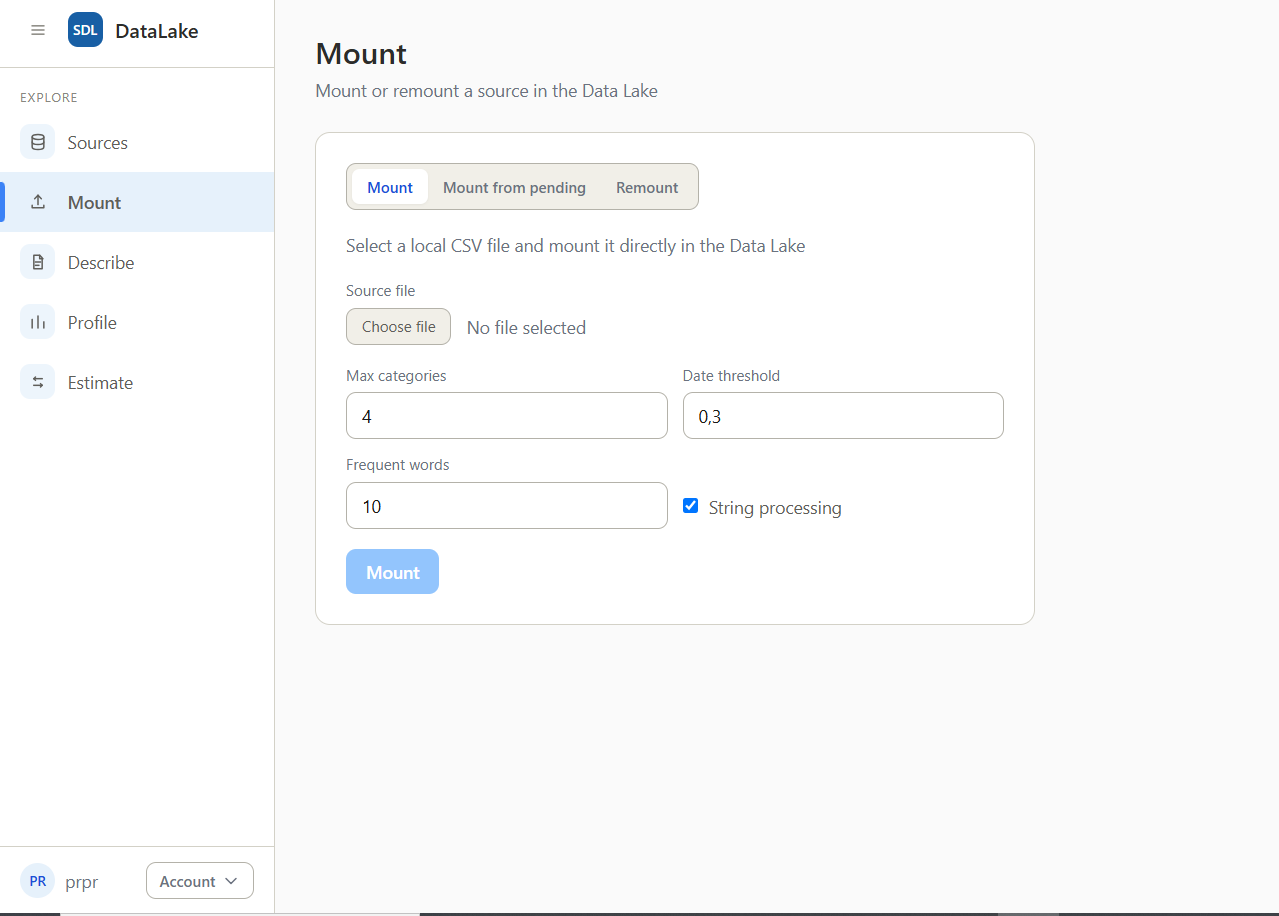
\includegraphics[width=0.85\textwidth]{images/cap. 6/mount.PNG}
    
    \caption{Interfaccia per le operazioni di mount e remount}
    \label{fig:immagini}

\end{figure}


\section{Analisi delle sorgenti}
\subsection*{Describe}

La pagina Describe permette di visualizzare le informazioni descrittive associate a una sorgente montata. L'interfaccia recupera l'elenco delle sorgenti disponibili e consente all'utente di selezionare quella da analizzare, utilizzandola successivamente per effettuare la richiesta al backend.

\noindent
Le informazioni restituite vengono organizzate distinguendo i dati generali della sorgente da quelli relativi ai singoli domini. La prima parte della visualizzazione riporta informazioni quali il nome della sorgente, l'utente che ne ha effettuato il caricamento, la data di caricamento, il numero di elementi e il numero di domini individuati.

\noindent
Una seconda parte è invece dedicata alla struttura della sorgente e mostra i domini individuati durante il processo di profilazione. Per ciascuno di essi vengono presentate le relative informazioni e, quando il dominio risulta mappato, il corrispondente livello del Knowledge Graph e il valore di completezza. La pagina permette quindi di ottenere una visione complessiva sia delle caratteristiche generali della sorgente sia della sua struttura e del relativo mapping semantico.

%*** screen di esempio della schermata describe ***

\begin{figure}[h]
    \centering
    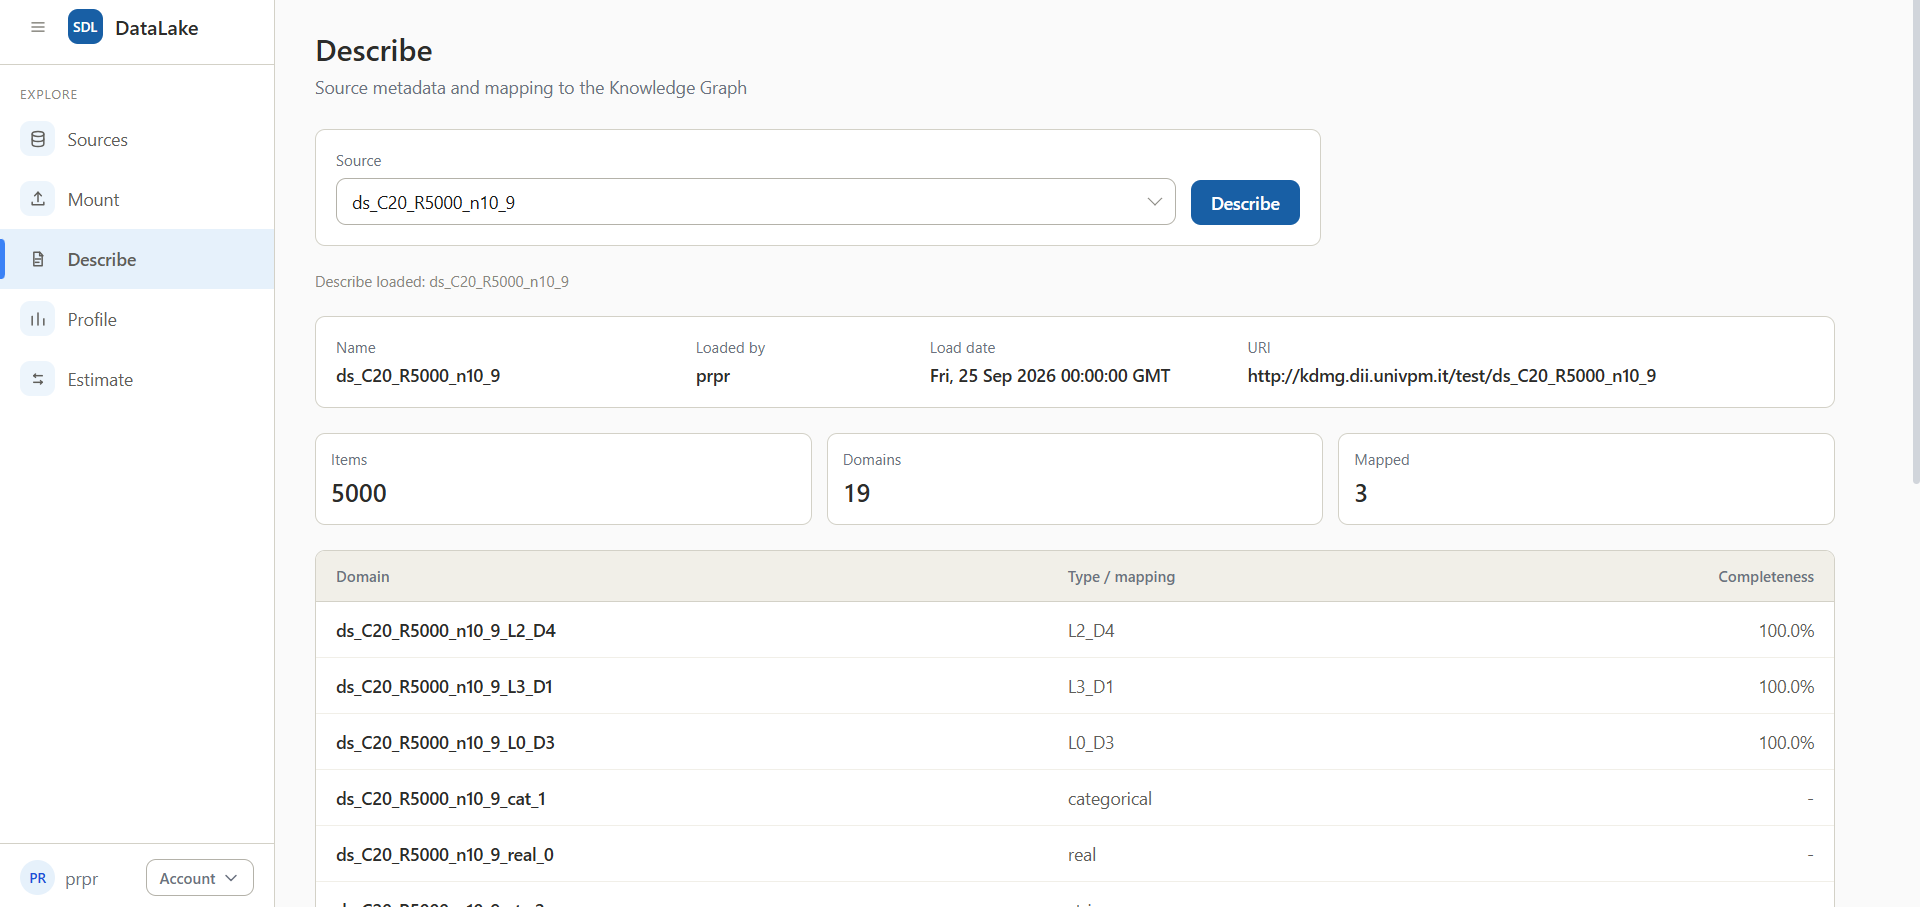
\includegraphics[width=0.9\linewidth]{images/cap. 6/describe.PNG}
    \caption{Visualizzazione delle informazioni relative a una sorgente}
    \label{fig:placeholder}
\end{figure}

\vspace{1cm}

\subsection*{Profile}

La pagina Profile consente di esaminare nel dettaglio il profilo dei dati contenuti in una sorgente. Dopo la selezione della sorgente, il frontend utilizza le informazioni ottenute tramite Describe per ricavarne i domini disponibili, permettendo all'utente di richiedere il profilo dell'intera sorgente oppure di limitare l'analisi a uno specifico dominio.

\noindent
È inoltre possibile richiedere l'operazione di roll-up per i domini per i quali questa risulta applicabile. La struttura dei dati restituiti dal backend varia in funzione della modalità selezionata: il profilo completo della sorgente, il profilo di un singolo dominio e le richieste che includono il roll-up possono produrre risposte organizzate in maniera differente. Il frontend gestisce tali differenze e riconduce i risultati a una rappresentazione utilizzabile in maniera uniforme dai componenti dell'interfaccia.

\begin{figure}[H]
    \centering
    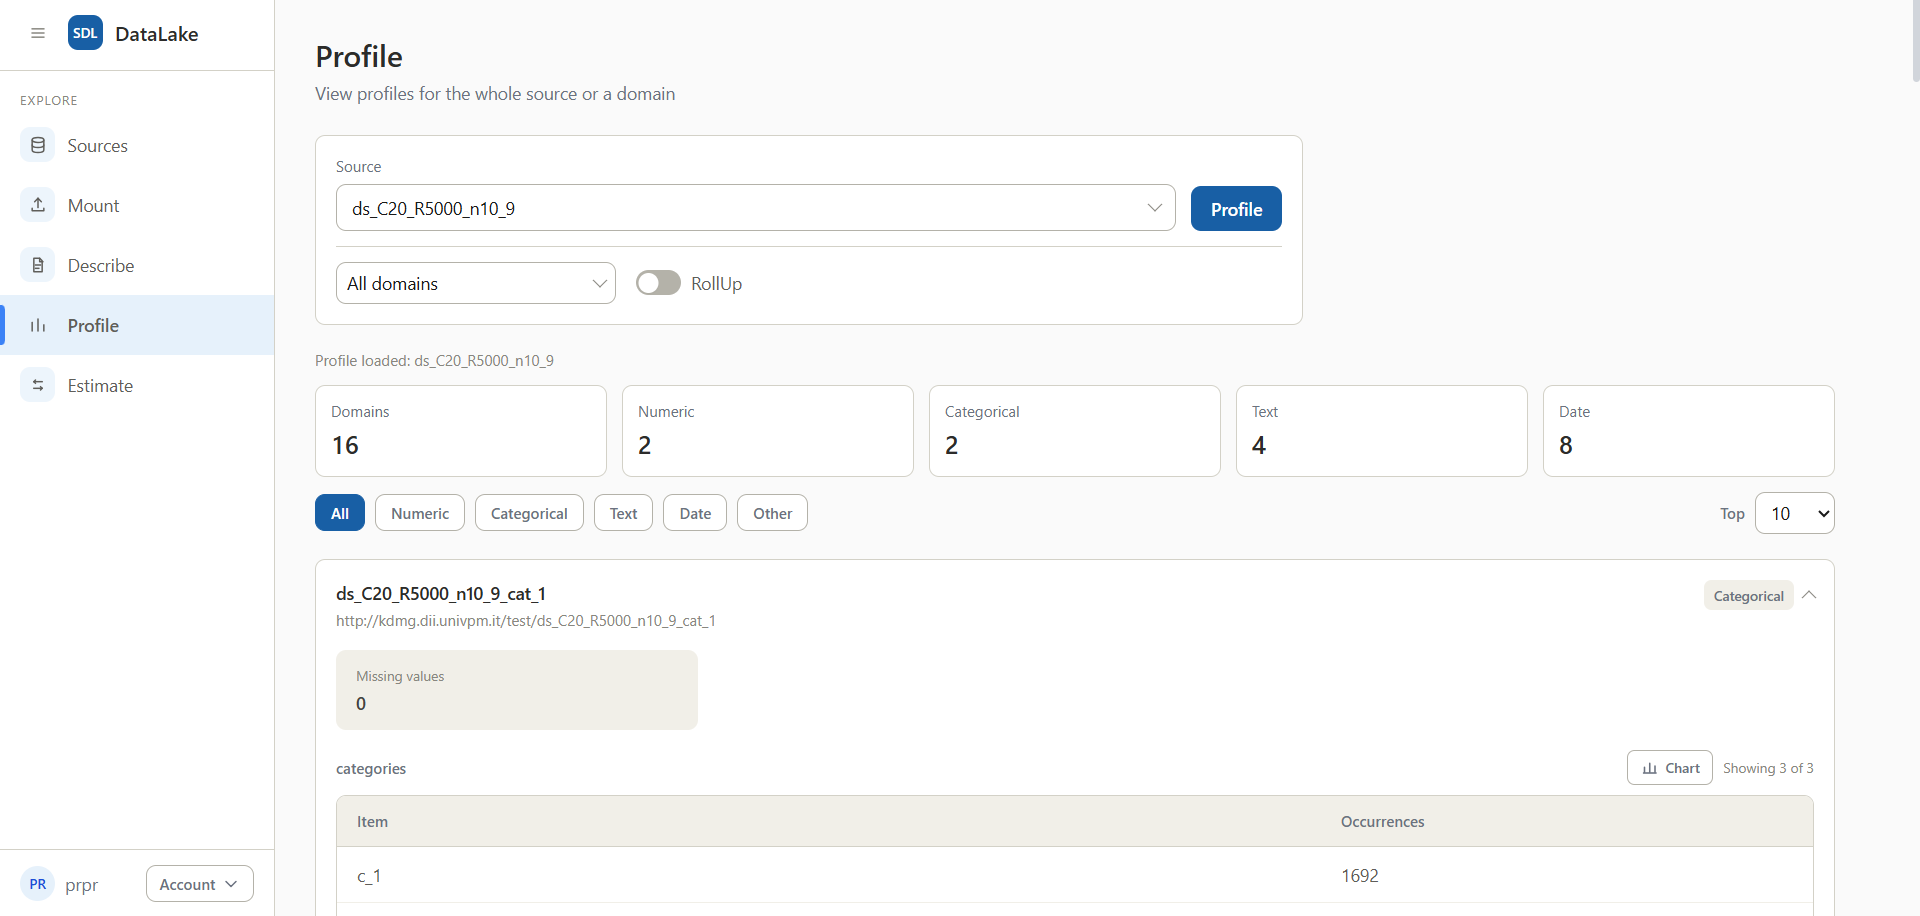
\includegraphics[width=0.9\linewidth]{images/cap. 6/profile1.PNG}
    \caption{Interfaccia per la visualizzazione dei profili di una sorgente}
    \label{fig:placeholder}
\end{figure}

\noindent
La visualizzazione viene successivamente adattata alle caratteristiche del profilo ottenuto, distinguendo differenti tipologie di dati, tra cui valori numerici, categorici, testuali, temporali o generici. Per le informazioni basate sulle frequenze è inoltre possibile utilizzare una rappresentazione tabellare oppure un grafico a barre, limitando il numero di elementi visualizzati quando necessario. 

%*** screen di esempio della schermata profile ***

\begin{figure}[H]
    \centering

    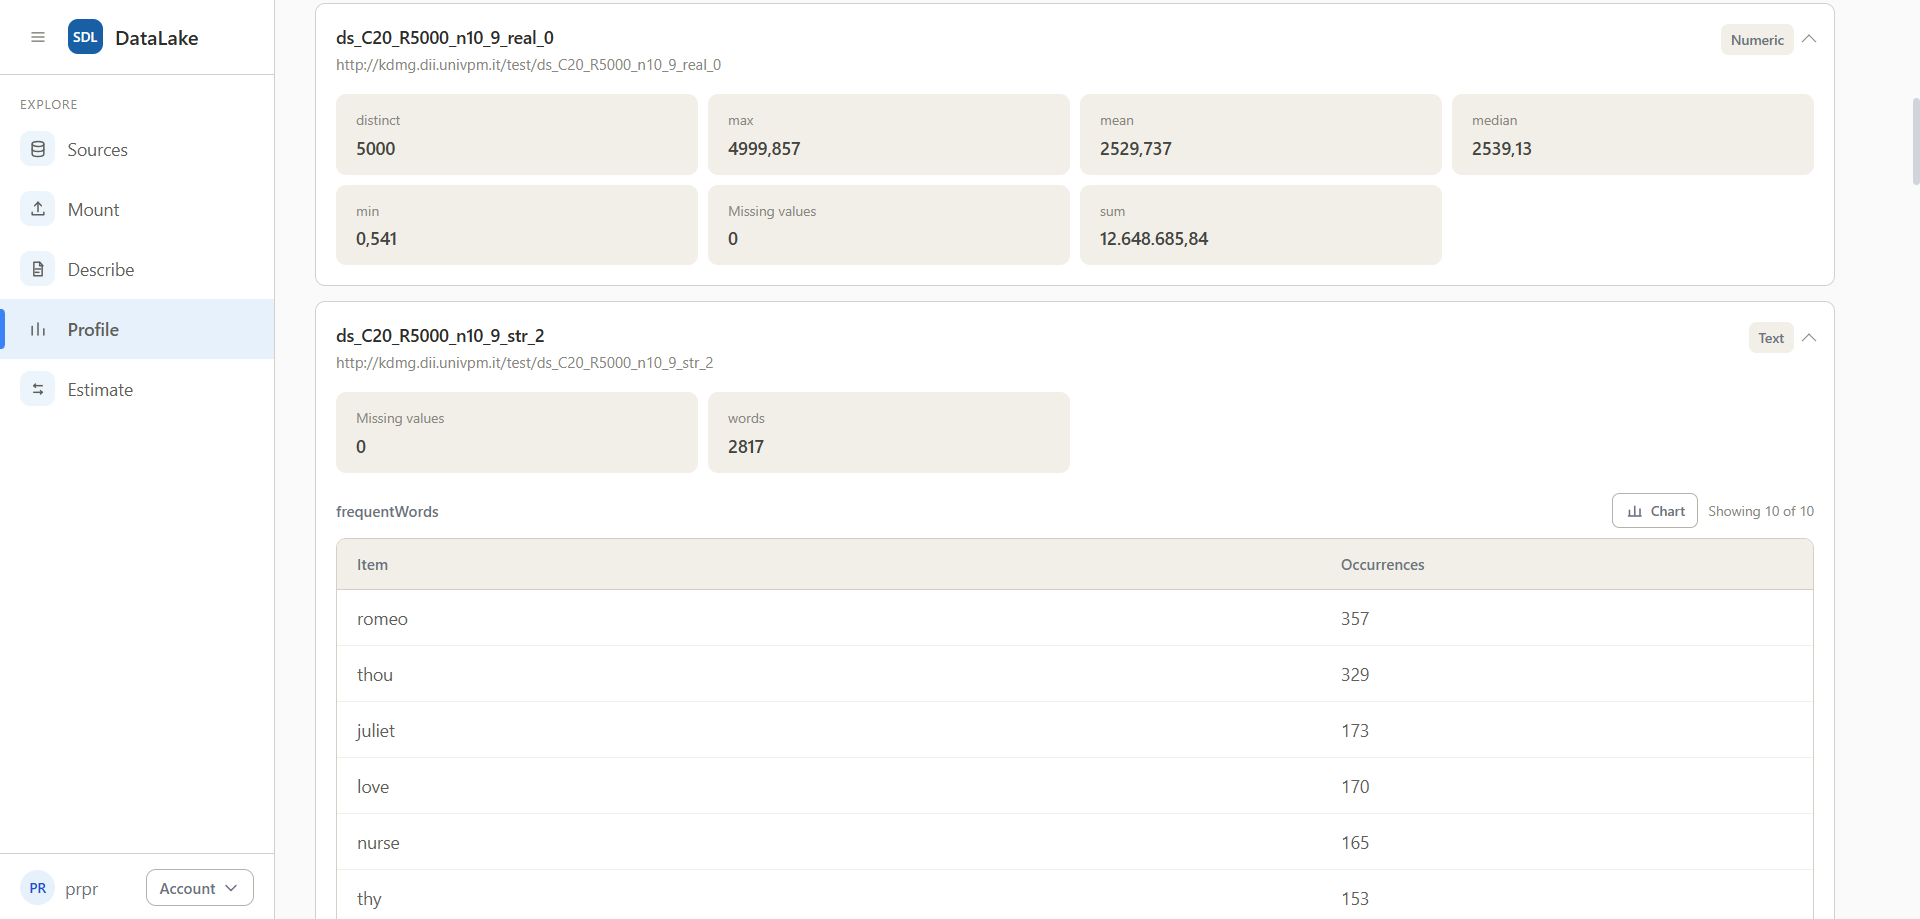
\includegraphics[width=0.8\textwidth]{images/cap. 6/profile2.PNG}

    \vspace{0.5cm}

    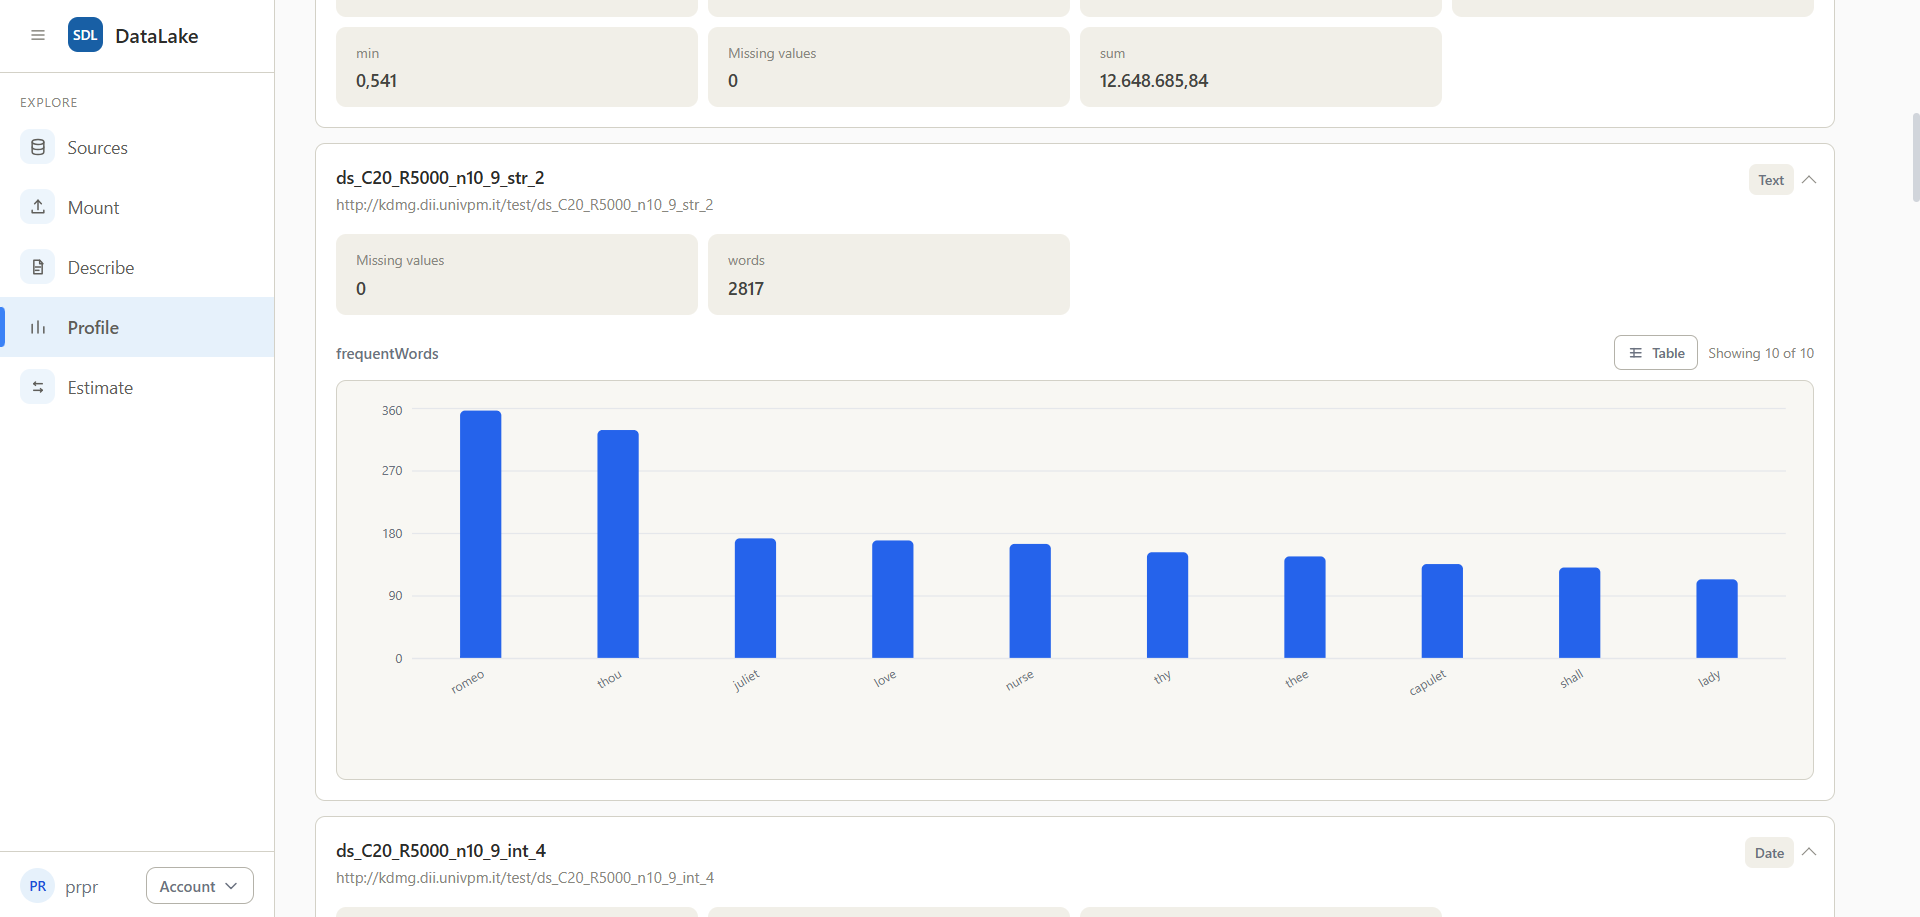
\includegraphics[width=0.8\textwidth]{images/cap. 6/profile3.PNG}

    \caption{Visualizzazione tabellare e grafica dei risultati del profiling}
    \label{fig:profile-results}
\end{figure}


\subsection*{Estimate}

La pagina Estimate permette di confrontare due sorgenti montate attraverso la funzionalità di stima della similarità fornita dal backend. L'utente seleziona le due sorgenti da confrontare tra quelle disponibili e il frontend utilizza tali informazioni per costruire la relativa richiesta.

\noindent
Il risultato del confronto viene elaborato e organizzato dall'interfaccia per evidenziare i livelli comuni individuati tra le due sorgenti e i relativi valori di similarità, insieme ai domini coinvolti nel confronto. Anche in questo caso la risposta del backend viene quindi trasformata in una rappresentazione più facilmente consultabile dall'utente.

\begin{figure}[H]
    \centering
    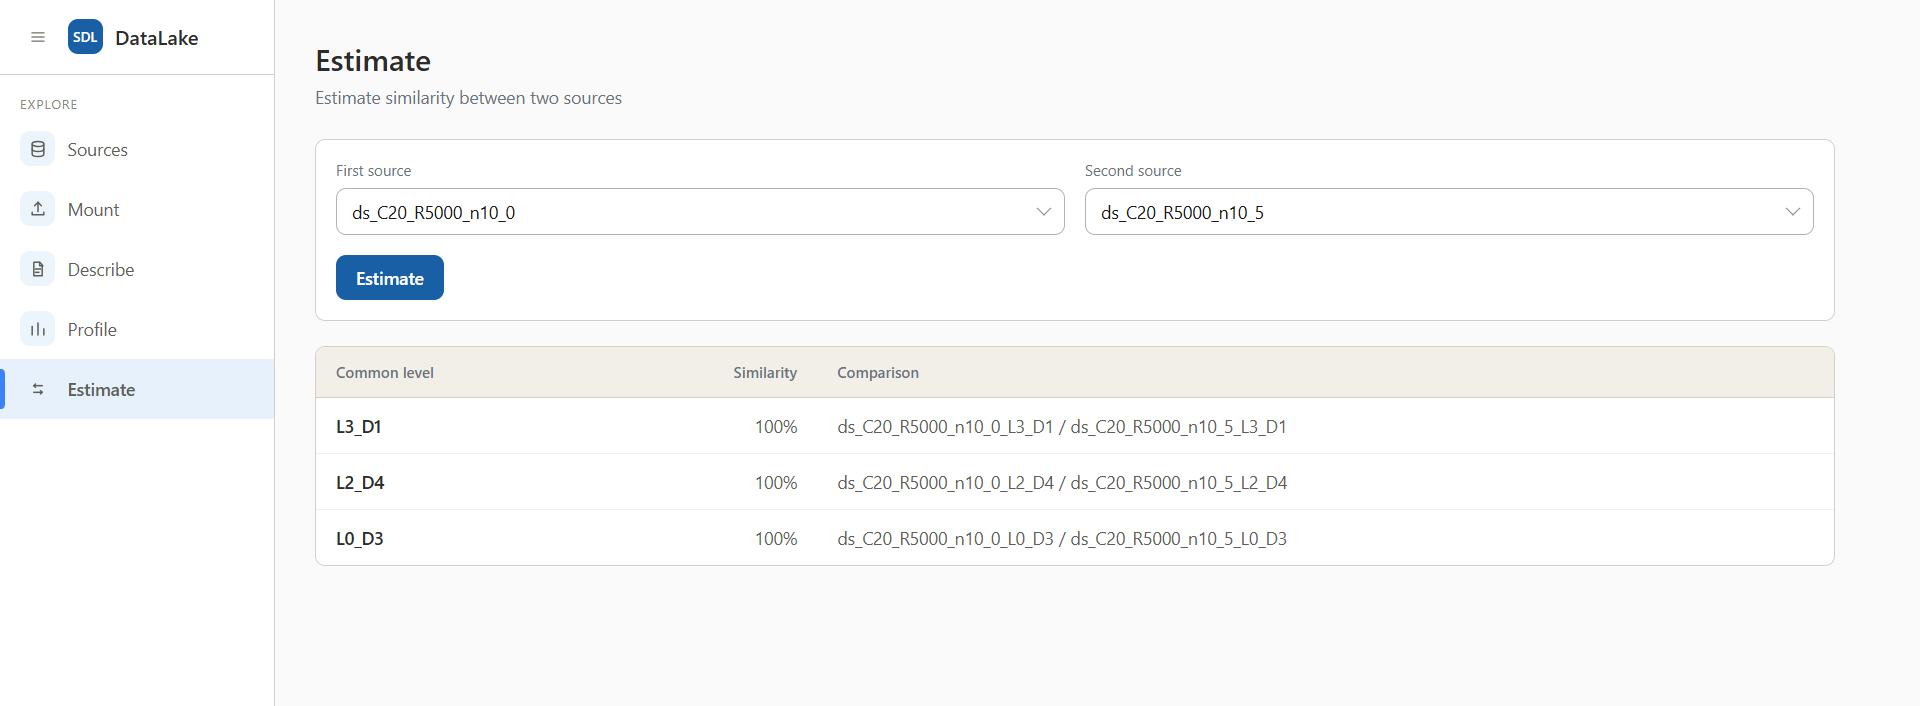
\includegraphics[width=0.9\linewidth]{images/cap. 6/estimate_2.png}
    \caption{Stima della similarità tra due sorgenti}
    \label{fig:placeholder}
\end{figure}

\section{Impostazioni} %da valutare (forse è meglio metterla, spiegando che ha come obiettivo l'essere pronta all'aggiuta di nuove funzionalità)

L'applicazione comprende una pagina dedicata alle impostazioni, accessibile dal menu dell'utente e pensata come punto centralizzato per le operazioni relative alla gestione dell'account che non appartengono direttamente alle funzionalità di analisi delle sorgenti. Nella versione attuale la sezione destinata all'utente ordinario contiene esclusivamente la funzionalità per la pulizia dei metadati associati alle proprie sorgenti.

\noindent
La pagina è stata mantenuta separata dalle funzionalità operative dell'applicazione in modo da poter essere estesa in futuro con ulteriori impostazioni senza modificare l'organizzazione delle pagine dedicate alla gestione e all'analisi delle sorgenti.

\section{Funzionalità amministrative}
%spiegare solo le differenze, e mettere una schermata di esempio

L'interfaccia dedicata all'amministratore estende le funzionalità disponibili per l'utente ordinario, permettendo di eseguire le principali operazioni anche sulle risorse appartenenti agli altri utenti del sistema. Le pagine dedicate alla gestione e all'analisi delle sorgenti mantengono una struttura analoga a quella già descritta, aggiungendo, dove necessario, la possibilità di selezionare l'utente sul quale eseguire l'operazione. Le richieste vengono quindi indirizzate ai corrispondenti endpoint amministrativi del backend.

%*** screen di esempio di schermata admin ***

\noindent
Oltre a tali estensioni, l'area amministrativa mette a disposizione alcune funzionalità specifiche, dedicate all'interrogazione diretta dei grafi RDF e alla gestione degli utenti.

\subsection{Console SPARQL}

La console SPARQL permette all'amministratore di eseguire direttamente query sul grafo RDF attraverso un editor integrato nell'interfaccia. Il testo della query viene inviato al relativo endpoint, che ne esegue l'elaborazione e restituisce il risultato al frontend.

\noindent
Dove possibile, il frontend ricava le variabili richieste dalla query e le utilizza per determinare le colonne della tabella nella quale vengono organizzati i risultati restituiti dal backend. In questo modo la struttura della tabella dei risultati viene costruita dinamicamente in funzione dell'interrogazione eseguita, senza richiedere una struttura predefinita per i risultati.

\noindent
La console mantiene inoltre una cronologia locale delle query eseguite, permettendo di recuperare e riutilizzare rapidamente interrogazioni precedenti. Sono presenti anche funzionalità di supporto, come la possibilità di copiare il contenuto della query negli appunti. L'interfaccia fornisce quindi uno strumento per interrogare direttamente i dati RDF e consultarne i risultati senza dover interagire manualmente con gli endpoint del backend.

\vspace{0.5cm}

\begin{figure}[H]
    \centering
    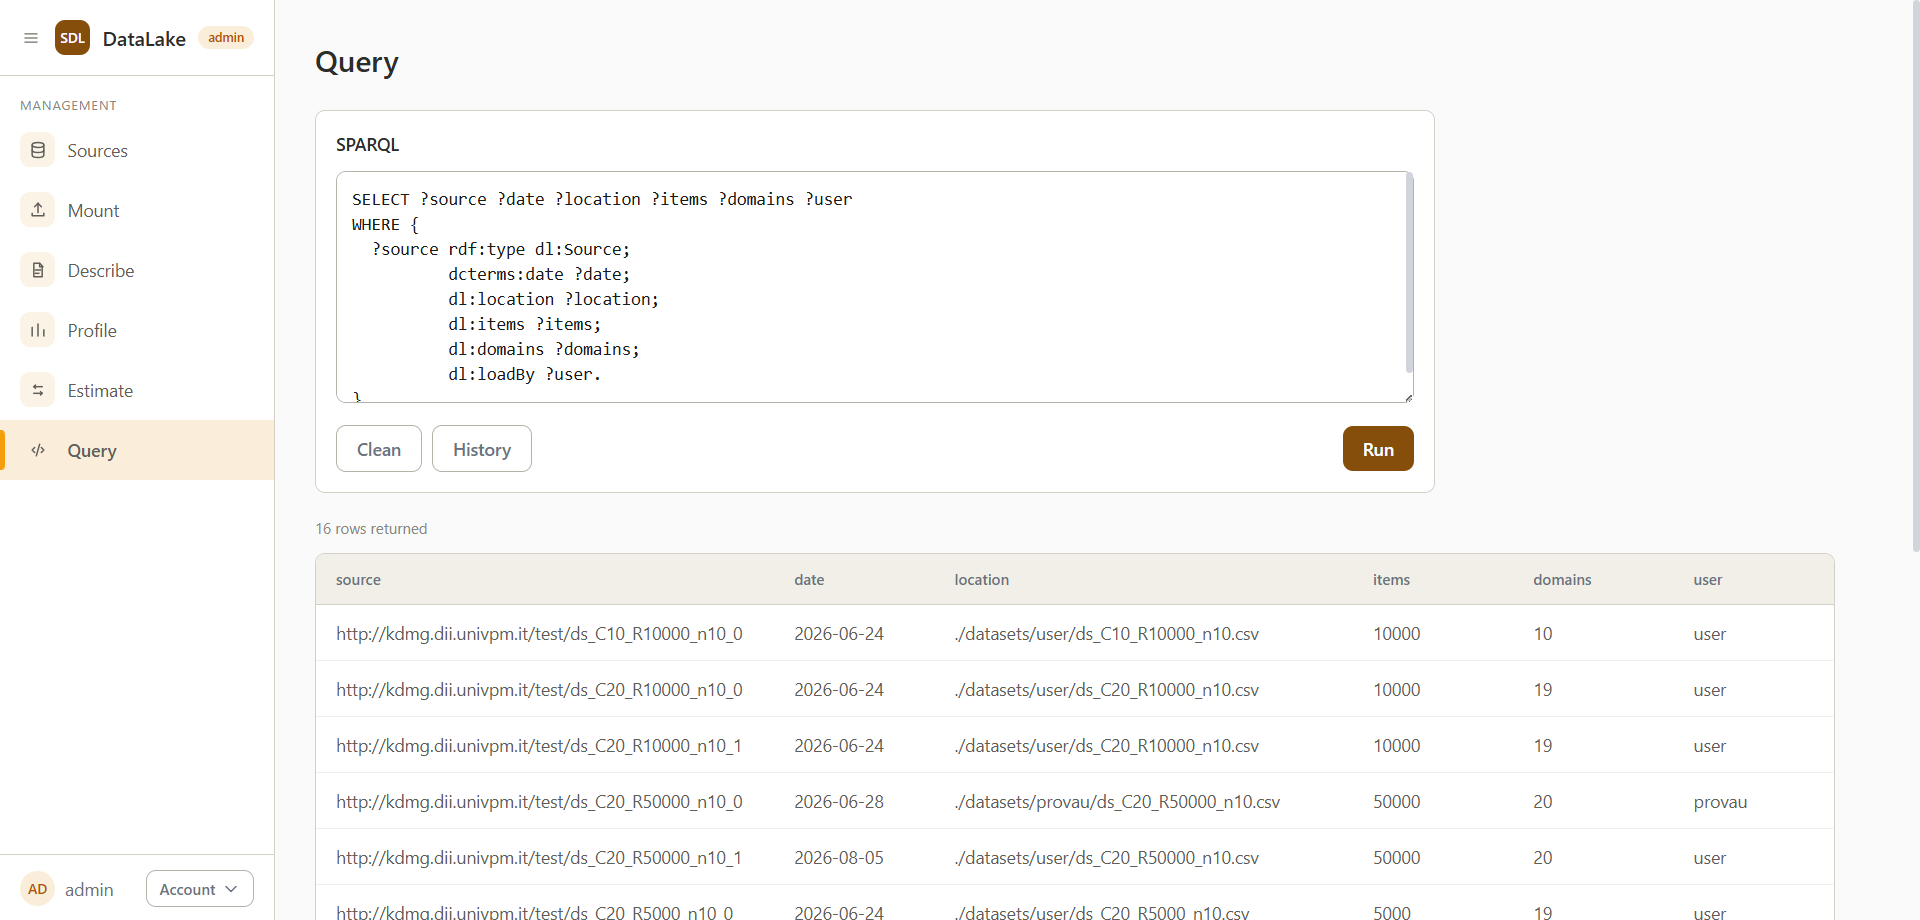
\includegraphics[width=0.8\linewidth]{images/cap. 6/console_query.PNG}
    \caption{Interfaccia della console SPARQL}
    \label{fig:placeholder}
\end{figure}

\vspace{2cm}

\subsection{Gestione utenti}
%la parte in settings

Per l'amministratore, la pagina delle impostazioni comprende anche una sezione dedicata alla gestione degli altri utenti registrati nel sistema. L'interfaccia presenta l'elenco degli utenti e associa a ciascuno le operazioni amministrative disponibili. In particolare, è possibile effettuare la pulizia dei metadati relativi a uno specifico utente oppure procedere all'eliminazione dell'utente stesso. 

\begin{figure}[H]
    \centering
    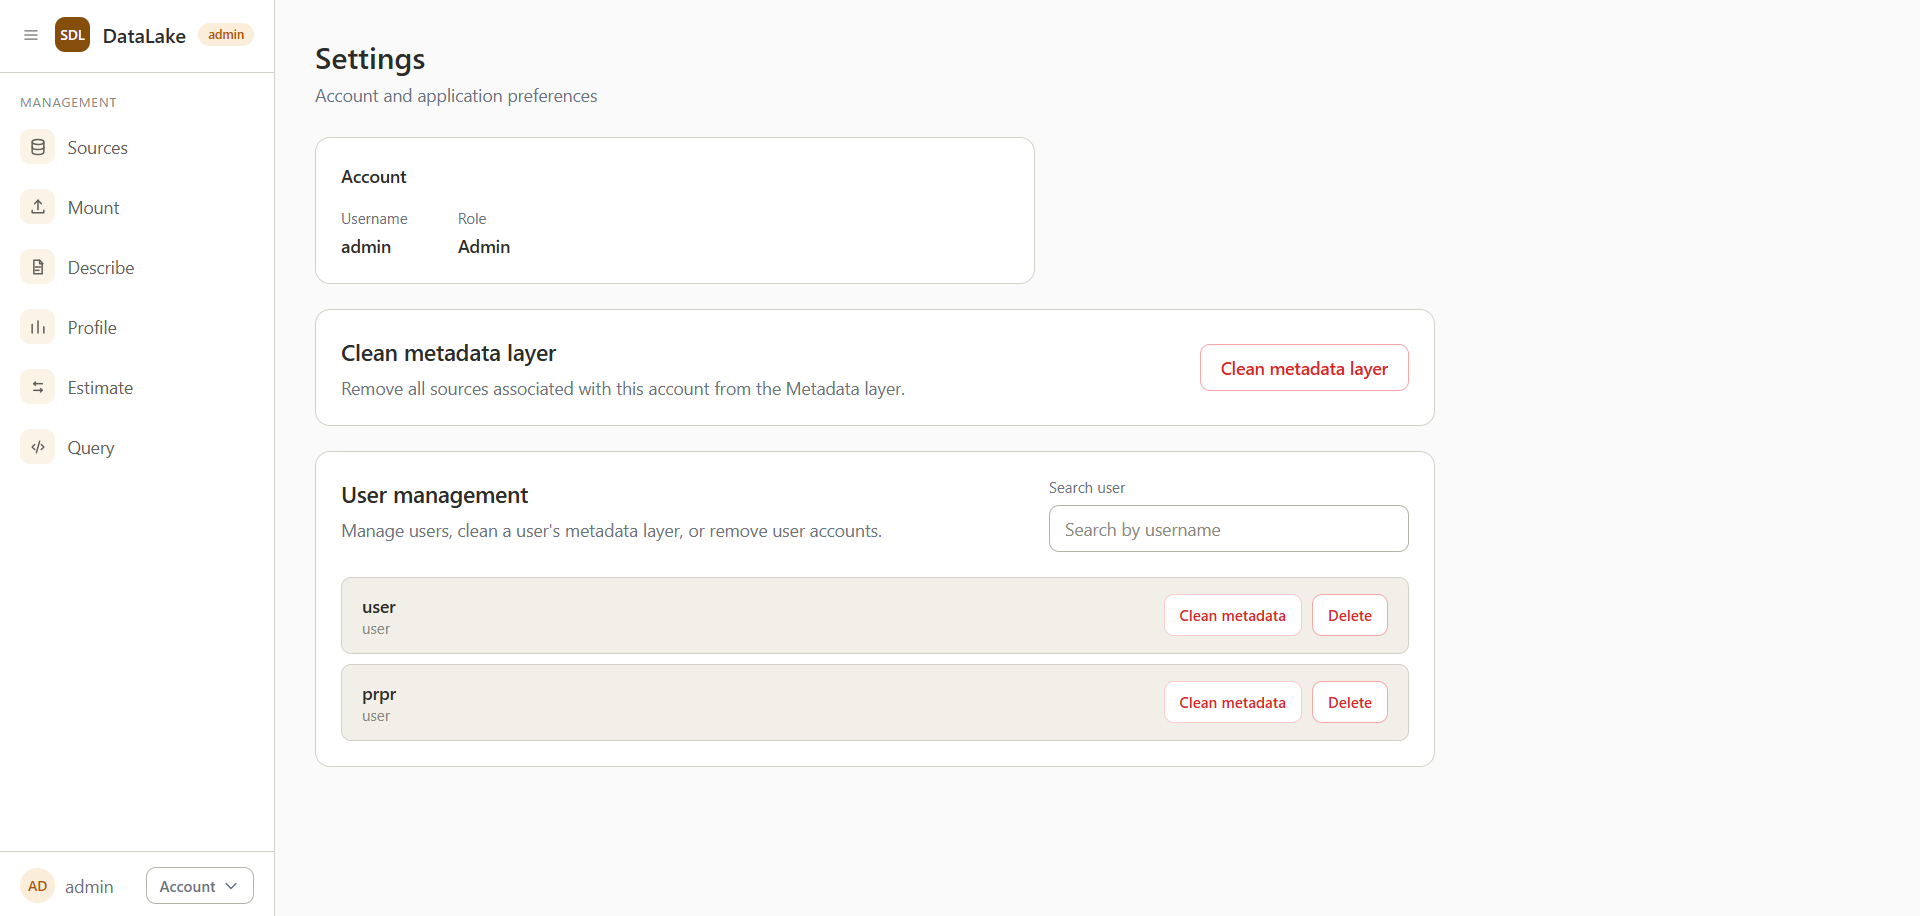
\includegraphics[width=0.8\linewidth]{images/cap. 6/admin_settings.PNG}
    \caption{Gestione degli utenti del sistema}
    \label{fig:placeholder}
\end{figure}

\chapter{Risultati}

Il lavoro svolto ha portato alla realizzazione di un'interfaccia web attraverso la quale è possibile accedere alle principali funzionalità offerte dal Semantic Data Lake. L'applicazione permette di gestire le sorgenti e utilizzare le operazioni di analisi messe a disposizione dal backend attraverso un ambiente grafico, differenziando le funzionalità disponibili in base al ruolo dell'utente autenticato.

\noindent
L'interfaccia consente di seguire le diverse fasi di gestione delle sorgenti, dal loro caricamento fino all'integrazione nel Data Lake, e di consultare in maniera organizzata le informazioni prodotte dalle operazioni di analisi. Le funzionalità amministrative permettono inoltre di estendere le operazioni alle risorse appartenenti agli altri utenti e forniscono strumenti specifici per la gestione del sistema e l'interrogazione dei grafi RDF.

\noindent
Lo sviluppo del frontend ha inoltre evidenziato la necessità di rendere più flessibile il ciclo di gestione delle sorgenti. L'estensione del backend ha permesso di separare il caricamento di un file dalla sua successiva integrazione nel Data Lake, consentendo di mantenere sul server sorgenti in attesa di mount e di elaborarle in un momento successivo. Tale modifica ha permesso di integrare nell'interfaccia un flusso di gestione più versatile rispetto a quello previsto dal sistema originario.

\noindent
Nel complesso, la soluzione sviluppata integra quindi le funzionalità del backend preesistente all'interno di un'interfaccia unificata, affiancandovi le estensioni introdotte durante il progetto e mantenendo separati il livello di presentazione e la logica applicativa del Semantic Data Lake.

\section{Limiti e possibili sviluppi futuri}

La soluzione sviluppata soddisfa gli obiettivi definiti per il progetto, ma presenta alcuni aspetti che potrebbero essere oggetto di ulteriori sviluppi, soprattutto nell'ottica di un utilizzo del sistema con un maggior numero di utenti, sorgenti e quantità di dati.

\noindent
Un primo limite riguarda la gestione dell'autenticazione e della sessione. Il backend mantiene centralmente le informazioni relative all'utente autenticato e non gestisce sessioni indipendenti per client differenti. Questa soluzione risulta adeguata al contesto di sviluppo e utilizzo considerato, ma non consente una corretta gestione di più utenti connessi contemporaneamente. Una possibile evoluzione consiste quindi nell'introduzione di un sistema di autenticazione e gestione delle sessioni adatto a un ambiente multiutente.

\noindent
Un secondo aspetto riguarda la persistenza dei dati applicativi. Le informazioni relative agli utenti vengono memorizzate in un file CSV, mentre i grafi RDF sono gestiti attraverso RDFLib e serializzati su file. All'aumentare del numero di utenti e della quantità di informazioni gestite, potrebbe risultare opportuno adottare sistemi di persistenza maggiormente adatti ad accessi concorrenti e a quantità di dati più elevate, valutando ad esempio l'utilizzo di un database per i dati applicativi e di un sistema di persistenza dedicato per i grafi RDF.

\noindent
Un ulteriore limite è rappresentato dalla natura sincrona delle operazioni di mount e profiling. L'elaborazione di una sorgente viene eseguita nell'ambito della richiesta HTTP e il client deve quindi attendere il completamento dell'intero processo. Con sorgenti di dimensioni maggiori potrebbe essere preferibile introdurre un meccanismo di elaborazione asincrona, nel quale le operazioni vengono gestite come job e il relativo stato può essere consultato dall'interfaccia durante l'esecuzione.

\noindent
Il sistema supporta inoltre esclusivamente sorgenti in formato CSV. Un possibile sviluppo futuro consiste nell'estendere il processo di caricamento e profiling ad altri formati di dati strutturati o semi-strutturati, permettendo al Data Lake di gestire una maggiore varietà di sorgenti.

\noindent
Infine, l'attuale processo di profiling viene eseguito localmente dal backend e non è progettato per l'elaborazione di dataset di dimensioni particolarmente elevate. Un'evoluzione del sistema potrebbe quindi riguardare l'ottimizzazione del processo di analisi e l'introduzione di modalità di elaborazione maggiormente scalabili, qualora fosse necessario gestire volumi di dati significativamente superiori a quelli considerati nel progetto.

\end{document}
